% !TEX program = xelatex
% עיצוב בהתאם לפורמט דו"ח פרויקט הגמר (Final Report format)
% Compile with: latexmk -xelatex main.tex
\documentclass[11pt,a4paper]{article}
\renewcommand{\labelitemi}{$\bullet$}

% — עמוד וריווח —
\usepackage[a4paper,left=25mm,right=25mm,top=20mm,bottom=25mm]{geometry}
\usepackage{setspace}
\onehalfspacing
\setlength{\emergencystretch}{2em}

% — חבילות עיצוב ומתמטיקה —
\usepackage{amsmath}
\usepackage{amssymb}
\usepackage{graphicx}
\usepackage{float}
\usepackage{listings}
\usepackage[dvipsnames]{xcolor}
\usepackage{booktabs,array}
\usepackage{pdfpages}

% — כיתובים (captions) בסגנון דו"ח הגמר —
\usepackage{caption}
\captionsetup{font=small,labelfont=bf,textfont=it,skip=6pt,justification=centering}

% — כותרות פרקים בכחול, בסגנון דו"ח הגמר —
\usepackage{titlesec}
\titleformat{\part}[display]{\centering\bfseries\huge\color{Blue}}{\partname~\thepart}{6pt}{}
\titlespacing*{\part}{0pt}{12pt}{20pt}
\titleformat{\section}[hang]{\bfseries\Large\color{Blue}}{\thesection}{1em}{}
\titlespacing*{\section}{0pt}{14pt}{8pt}
\titleformat{\subsection}[hang]{\bfseries\large\color{Blue}}{\thesubsection}{1em}{}
\titleformat{\subsubsection}[hang]{\bfseries\normalsize\color{Blue}}{\thesubsubsection}{1em}{}

% — כותרת תחתונה: מספר עמוד במרכז —
\usepackage{fancyhdr}
\pagestyle{fancy}
\fancyhf{}
\renewcommand{\headrulewidth}{0pt}
\fancyfoot[C]{\thepage}

% — קישורים (חייב להיטען לפני polyglossia/bidi) —
\usepackage[colorlinks=true,linkcolor=black,urlcolor=Blue,citecolor=black]{hyperref}

% — הגדרת שפה ותמיכה בעברית —
\usepackage{polyglossia}
\setmainlanguage{hebrew}
\setotherlanguage{english}

% — הגדרת גופנים —
\setmainfont{TeX Gyre Termes}
\newfontfamily\hebrewfont[Script=Hebrew]{David CLM}
\newfontfamily\hebrewfontsf[Script=Hebrew]{Miriam CLM}
\newfontfamily\hebrewfonttt[Script=Hebrew]{Miriam Mono CLM}

% — הגדרת עיצוב עבור בלוקים של קוד —
\lstset{
    backgroundcolor=\color{gray!5},
    basicstyle=\small\ttfamily,
    breaklines=true,
    frame=single,
    numbers=left,
    numberstyle=\tiny\color{gray},
    keywordstyle=\color{blue},
    commentstyle=\color{green!60!black},
    stringstyle=\color{purple},
    keepspaces=true
}

% — קישורי GitHub של הפרויקט —
\newcommand{\repourl}{https://github.com/ThEpiCake/Robot_Navigation_and_Control}
\newcommand{\repotext}{\textenglish{\texttt{github.com/ThEpiCake/Robot\_Navigation\_and\_Control}}}

\begin{document}
% ==================== דף שער (TITLE PAGE) ====================
\pagenumbering{gobble}
\begin{titlepage}
    \centering
    % שורת הלוגואים והטקסט ביניהם
    \noindent
    \begin{minipage}[c]{0.2\textwidth}
        \centering
        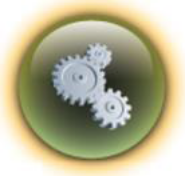
\includegraphics[width=\linewidth]{mech_logo.png}
    \end{minipage}%
    \hfill
    \begin{minipage}[c]{0.55\textwidth}
        \centering
        {\large \textbf{אוניברסיטת בן-גוריון בנגב}\par}
        \vspace{2pt}
        {\large \textbf{הפקולטה למדעי ההנדסה}\par}
        \vspace{2pt}
        {\large \textbf{המחלקה להנדסת מכונות}\par}
    \end{minipage}%
    \hfill
    \begin{minipage}[c]{0.2\textwidth}
        \centering
        
\includegraphics[width=\linewidth]{bgu_logo.png}
    \end{minipage}

    \vspace{2.6cm}

    {\huge\bfseries ניווט ובקרת רובוטים\par}
    \vspace{0.35cm}
    {\LARGE מיני-פרויקט — דו"ח סופי\par}
    \vspace{0.35cm}
    {\large קורס \textenglish{362-2-5481} \par}

    \vspace{1.6cm}

    {\renewcommand{\arraystretch}{1.5}
    \begin{tabular}{r l l}
    \textbf{מגישים:} & איתי ברון & \textenglish{209438910} \\
                     & רועי זהבי & \textenglish{209146216} \\
    \textbf{מנחה:}   & פרופ' אמיר שפירא & \\
    \textbf{תאריך הגשה:} & \textenglish{6.7.2026} & \\
    \end{tabular}}

    \vfill

    % ==== קישור GitHub — כל קוד המקור והחומרים הנלווים ====
    \rule{0.85\linewidth}{0.4pt}\\[10pt]
    {\normalsize\bfseries קוד המקור המלא, המצגת, המאמר וסרטוני הסימולציה — \textenglish{GitHub}:\par}
    \vspace{4pt}
    {\small \href{\repourl}{\repotext}\par}
    \vspace{6pt}
    {\small
    חלק 1 — זרוע רובוטית:
    \href{\repourl/tree/main/src}{\textenglish{\texttt{src/}}}
    \quad$\vert$\quad
    חלק 2 — רחפן אוטונומי:
    \href{\repourl/tree/main/swarm_project/ros2_ws/src}{\textenglish{\texttt{swarm\_project/ros2\_ws/src/}}}
    \par}
\end{titlepage}
% =============================================================
% תוכן עניינים, רשימת איורים ורשימת טבלאות
\newpage
\pagenumbering{roman}
\setcounter{page}{1}
\tableofcontents
\newpage
\begingroup\small
\listoffigures
\newpage
\listoftables
\endgroup
\newpage
\pagenumbering{arabic}
\setcounter{page}{1}

% ==================== תחילת חלק 1 ====================
\part{מודל דינמי, סימולציה ובקרה}

\section{הצגת המערכת והבעיה (\textenglish{The Problem Used in the Simulations})}

\subsection{תיאור מניפולטור המטרה (\textenglish{Robot Description})}
עבור פרויקט זה תוכנן ומומש מניפולטור רובוטי בעל 6 דרגות חופש (\textenglish{DOF}) בתצורת \textenglish{R-P-P-R-R-R} מותאמת אישית (\texttt{custom\_rpp\_zyz\_robot}). הרובוט תוכנן לבצע משימות איסוף והנחה (\textenglish{Pick and Place}) במרחבים צפופים כגון מדפי ספרים.

המבנה הקינמטי של הרובוט מוגדר על ידי וקטור המשתנים הבא:
\begin{equation}
q = \begin{bmatrix}\theta_1 & d_1 & d_2 & \theta_4 & \theta_5 & \theta_6\end{bmatrix}^T
\end{equation}

כאשר:
\begin{itemize}
    \item $\theta_1, \theta_4, \theta_5, \theta_6$ הם מפרקים סיבוביים (\textenglish{Revolute}).
    \item $d_1, d_2$ הם מפרקים פריזמטיים (\textenglish{Prismatic}).
\end{itemize}

חלוקת המפרקים הפיזית היא כדלקמן:
\begin{itemize}
    \item $\theta_1$ - מפרק בסיס סובב (\textenglish{Revolute Yaw}): סיבוב סביב ציר $Z$ הגלובלי המאפשר צידוד של המערכת כולה.
    \item $d_1$ - זרוע טלסקופית ראשונה (\textenglish{Prismatic}): תנועה קווית (הגבהה) לאורך ציר $Z$ המקומי, המאפשרת שינוי גובה המערכת.
    \item $d_2$ - זרוע טלסקופית שנייה (\textenglish{Prismatic}): לאחר הטיה קבועה של 135 מעלות כלפי מטה, ממוקמת זרוע טלסקופית נוספת המאפשרת חדירה לעומק המרחב.
    \item \textbf{פרק כף יד כדורי} (\textenglish{Spherical Wrist} - $\theta_4, \theta_5, \theta_6$): מפרקים סובבים בתצורת Z-Y-Z. ציריהם נחתכים בנקודה אחת, מה שמאפשר להפריד את חישוב המיקום מחישוב האוריינטציה של קצה האיבר (\textenglish{End-Effector}).
\end{itemize}
בנוסף, בקצה הרובוט מורכב גריפר בעל אצבעות קשיחות באורך 6 ס"מ.

\begin{figure}[h]
    \centering
    % שים לב: תמונה זו לא הופיעה בצילום המסך. אנא ודא שהיא קיימת בתיקיית results בשם זה.
    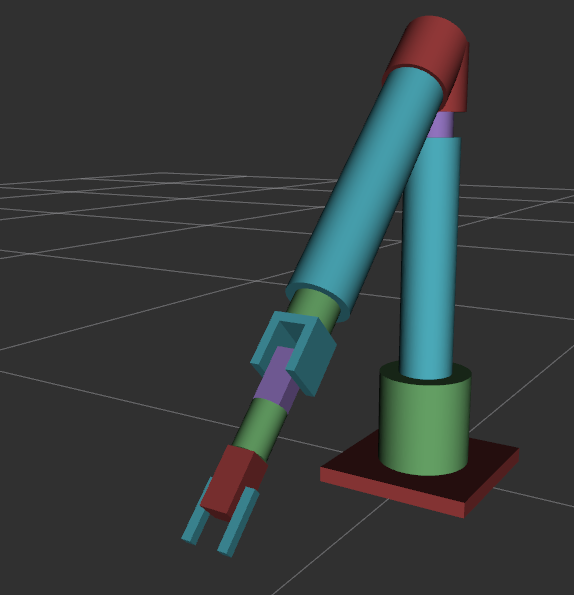
\includegraphics[width=0.6\textwidth]{../results/gripper_shelf.png}
    \caption{מבנה הגריפר בתצורת Z-Y-Z}
    \label{fig:gripper_shelf}
\end{figure}

\begin{figure}[h]
    \centering
    % שים לב: תמונה זו לא הופיעה בצילום המסך. אנא ודא שהיא קיימת בתיקיית results בשם זה.
    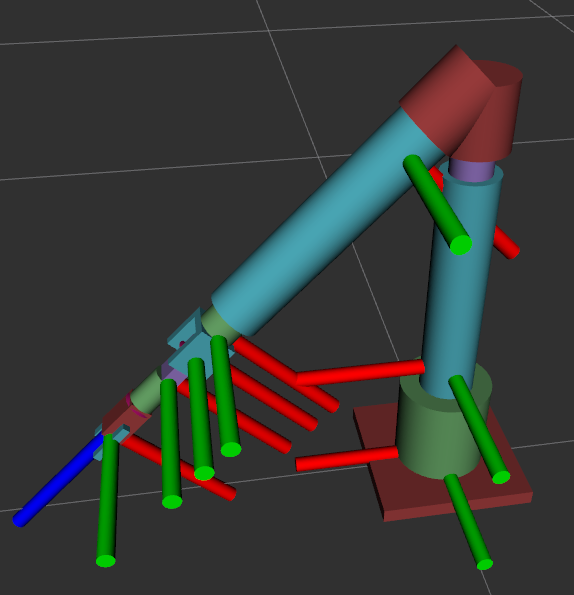
\includegraphics[width=0.6\textwidth]{../results/robot_general.png}
    \caption{תמונה כללית של הרובוט ב-\textenglish{RViz} המציגה את תצורתו המלאה.}
    \label{fig:robot_general}
\end{figure}

\subsection{תיאור משימת הסימולציה}
סביבת הסימולציה (\textenglish{Gazebo}) מורכבת מהרובוט ומדף ספרים כפול בעל חציצה קשיחה. המטרה היא להעביר את קצה הזרוע ממצב מנוחה התחלתי במדף התחתון לנקודת יעד במדף העליון, ללא התנגשות.
\begin{itemize}
    \item \textbf{נקודת ההתחלה (A):} $(X=0.455, Y=-0.1, Z=0.150)$.
    \item \textbf{נקודת היעד (B):} $(X=0.50, Y=-0.3, Z=0.32)$.
\end{itemize}

\subsection{מודל קינמטי (\textenglish{Kinematic Model})}

\textbf{גבולות מפרקים (\textenglish{Joint Limits}):} \\
על מנת להבטיח תנועה בטוחה ולמנוע התנגשויות עצמיות, הוגדרו גבולות המפרקים הבאים (על בסיס ההגדרות ב-\textenglish{URDF}):
\begin{align*}
0 \leq d_1 \leq 0.255 \, [m], \quad 0 \leq d_2 \leq 0.255 \, [m] & \quad \text{מפרקים פריזמטיים:} \\
-\pi \leq \theta_1, \theta_4, \theta_6 \leq \pi, \quad -\frac{\pi}{2} \leq \theta_5 \leq \frac{\pi}{2} & \quad \text{מפרקים סובבים:}
\end{align*}

\textbf{קינמטיקה ישירה (\textenglish{Forward Kinematics}):} \\
הקינמטיקה הישירה מחשבת את הטרנספורמציה $^0T_8$ מבסיס הרובוט לקצה ה-EE כפונקציה של וקטור המפרקים $q$. השרשרת הקינמטית מתוארת על ידי מכפלת מטריצות הטרנספורמציה הבסיסיות:
\begin{equation}
^0T_8 = {^0A_1} \cdot {^1A_2} \cdot {^2A_3} \cdot {^3A_4} \cdot {^4A_5} \cdot {^5A_6} \cdot {^6A_7} \cdot {^7A_8}
\end{equation}

הקבועים הגיאומטריים (אורכי החוליות) המופיעים במטריצות נגזרו ישירות מה-\textenglish{URDF}:
\begin{table}[H]
\centering
\begin{tabular}{ccc}
\toprule
\textbf{מטריצה} & \textbf{משמעות פיזיקלית} & \textbf{ערך [m]} \\
\midrule
$^0A_1$ & גובה מנוע הבסיס מעל הקרקע & 0.02 \\
$^1A_2$ & אופסט קבוע של זרוע 1 + נסיעת $d_1$ & $0.15 + d_1$ \\
$^2A_3$ & גובה המכלול הנוטה (ציר הכיפוף) & 0.38 \\
$^3A_4$ & אופסט קבוע של זרוע 2 + נסיעת $d_2$ & $0.11 + d_2$ \\
$^4A_5$ & אורך הזרוע הטלסקופית הפנימית & 0.30 \\
$^5A_6$ & רוחב ציר כף היד (wrist\textunderscore{}z1 $\to$ wrist\textunderscore{}y) & 0.04 \\
$^6A_7$ & גובה מרכז כף היד (wrist\textunderscore{}y $\to$ wrist\textunderscore{}z2) & 0.05 \\
$^7A_8$ & אורך הגריפר עד קצה האיבר & 0.11 \\
\bottomrule
\end{tabular}
\caption{הקבועים הגיאומטריים של השרשרת הקינמטית, כפי שנגזרו מה-\textenglish{URDF}.}
\label{tab:geom_constants}
\end{table}

המטריצה $^2A_3$ קבועה ואינה תלויה במשתני המפרקים, שכן היא מייצגת הטיה קשיחה של $135^{\circ}$ סביב ציר $Y$. הרוטציה $R_y(135^{\circ})$ נותנת $\cos(135^{\circ})=-\frac{\sqrt{2}}{2}$ ו-$\sin(135^{\circ})=\frac{\sqrt{2}}{2}$, ומכאן הערכים המופיעים בשורות 1 ו-3 של המטריצה.

כאשר המטריצות מוגדרות כך (עבור $C_i = \cos(\theta_i)$, $S_i = \sin(\theta_i)$):
\begin{equation*}
^0A_1 = \begin{bmatrix} C_1 & -S_1 & 0 & 0 \\ S_1 & C_1 & 0 & 0 \\ 0 & 0 & 1 & 0.02 \\ 0 & 0 & 0 & 1 \end{bmatrix}, \quad
^1A_2 = \begin{bmatrix} 1 & 0 & 0 & 0 \\ 0 & 1 & 0 & 0 \\ 0 & 0 & 1 & 0.15 + d_1 \\ 0 & 0 & 0 & 1 \end{bmatrix}
\end{equation*}

\begin{equation*}
^2A_3 = \begin{bmatrix} -\frac{\sqrt{2}}{2} & 0 & \frac{\sqrt{2}}{2} & 0 \\ 0 & 1 & 0 & 0 \\ -\frac{\sqrt{2}}{2} & 0 & -\frac{\sqrt{2}}{2} & 0.38 \\ 0 & 0 & 0 & 1 \end{bmatrix}, \quad
^3A_4 = \begin{bmatrix} 1 & 0 & 0 & 0 \\ 0 & 1 & 0 & 0 \\ 0 & 0 & 1 & 0.11 + d_2 \\ 0 & 0 & 0 & 1 \end{bmatrix}
\end{equation*}

\begin{equation*}
^4A_5 = \begin{bmatrix} C_4 & -S_4 & 0 & 0 \\ S_4 & C_4 & 0 & 0 \\ 0 & 0 & 1 & 0.30 \\ 0 & 0 & 0 & 1 \end{bmatrix}, \quad
^5A_6 = \begin{bmatrix} C_5 & 0 & S_5 & 0 \\ 0 & 1 & 0 & 0 \\ -S_5 & 0 & C_5 & 0.04 \\ 0 & 0 & 0 & 1 \end{bmatrix}
\end{equation*}

\begin{equation*}
^6A_7 = \begin{bmatrix} C_6 & -S_6 & 0 & 0 \\ S_6 & C_6 & 0 & 0 \\ 0 & 0 & 1 & 0.05 \\ 0 & 0 & 0 & 1 \end{bmatrix}, \quad
^7A_8 = \begin{bmatrix} 1 & 0 & 0 & 0 \\ 0 & 1 & 0 & 0 \\ 0 & 0 & 1 & 0.11 \\ 0 & 0 & 0 & 1 \end{bmatrix}
\end{equation*}

\textbf{קינמטיקה הפוכה (\textenglish{Inverse Kinematics}):} \\
מטרת ה-IK היא למצוא את וקטור המפרקים $q$ בעבור יעד קצה נתון המאופיין על ידי מיקום $p$ ואוריינטציה $R$:
\begin{equation}
^0T_8(q) = \begin{bmatrix} R & p \\ 0 & 1 \end{bmatrix}
\end{equation}

הודות למבנה פרק כף היד הכדורי, הפתרון מבוסס על הפרדה קינמטית (\textenglish{Kinematic Decoupling}) המחלקת את הבעיה לשני שלבים:

\textbf{שלב 1: מיקום (חישוב $\theta_1, d_1, d_2$)} \\
מיקום מרכז פרק כף היד הכדורי, $P_c$, נגזר ממיקום קצה הזרוע לאחור לאורך ציר ה-$Z$ המקומי של הגריפר:
\begin{equation}
P_c = p - (a_7+a_8) \cdot R \hat{z}, \quad \hat{z}=\begin{bmatrix}0\\0\\1\end{bmatrix}
\end{equation}
כאשר $(a_7+a_8) = 0.05+0.11 = 0.16\,\text{m}$ הוא המרחק הקבוע מציר פרק כף היד הכדורי לקצה האיבר.

מכאן נחלץ את ערכי המפרקים על ידי השוואה לקינמטיקה הישירה של תת-השרשרת:
\begin{align}
\theta_1 &= \operatorname{atan2}(y_c, x_c) \nonumber \\
K &= \sqrt{x_c^2 + y_c^2} \implies d_2 = \sqrt{2}K - 0.45 \nonumber \\
d_1 &= z_c + \frac{\sqrt{2}}{2}d_2 + \frac{45\sqrt{2}}{200} - \frac{11}{20}
\end{align}
הקבועים בנוסחאות אלו נגזרים ישירות מהשרשרת הקינמטית: $0.45 = a_4+a_5+a_6 = 0.11+0.30+0.04$, ו-$0.55 = a_1+a_2+a_3 = 0.02+0.15+0.38$. שילוב מטריצות $^0A_1$ עד $^3A_4$ מוביל לפתרון הסגור הנ"ל ללא צורך בחיפוש איטרטיבי.

\textbf{שלב 2: אוריינטציה (חישוב $\theta_4, \theta_5, \theta_6$)} \\
מטריצת הרוטציה הנדרשת עבור פרק כף היד מחושבת על ידי $R_{47} = R_{04}^T \cdot R$. במודל \textenglish{Z-Y-Z}, במקרה הלא-סינגולרי ($s_5 \neq 0$), נבחר הענף החיובי:
\begin{align}
s_5 &= \sqrt{r_{13}^2 + r_{23}^2} \nonumber \\
\theta_5 &= \operatorname{atan2}(s_5, r_{33}) \nonumber \\
\theta_4 &= \operatorname{atan2}\left(\frac{r_{23}}{s_5}, \frac{r_{13}}{s_5}\right) \nonumber \\
\theta_6 &= \operatorname{atan2}\left(\frac{r_{32}}{s_5}, \frac{-r_{31}}{s_5}\right)
\end{align}
עבור המקרה הסינגולרי ($s_5 = 0$), הוגדרו המפרקים כ-$\theta_4=0, \theta_5=0, \theta_6=0$ לשם פישוט ויציבות הפתרון.


\section{מודל דינמי ומשוואות התנועה (\textenglish{Dynamical Equations of Motion})}
המודל הדינמי של המניפולטור מתאר את הקשר בין הכוחות והמומנטים המופעלים על המפרקים ($\tau$) לבין תנועת הרובוט ($q, \dot{q}, \ddot{q}$). לאור המורכבות הקינמטית של הרובוט, משוואות התנועה פותחו באופן סימבולי באמצעות גישת אוילר-לגראנז' (\textenglish{Euler-Lagrange}).

\subsection{גישת אוילר-לגראנז' (\textenglish{Euler-Lagrange Formulation})}
הפונקציה הלגראנג'ית של המערכת מוגדרת כהפרש בין האנרגיה הקינטית לאנרגיה הפוטנציאלית:
\begin{equation}
\mathcal{L}(q, \dot{q}) = T(q, \dot{q}) - V(q)
\end{equation}
כאשר $T = \frac{1}{2}\dot{q}^T M(q)\dot{q}$ היא האנרגיה הקינטית. משוואות התנועה נגזרות על פי כלל:
\begin{equation}
\frac{d}{dt}\frac{\partial \mathcal{L}}{\partial \dot{q}_i} - \frac{\partial \mathcal{L}}{\partial q_i} = \tau_i, \quad i = 1,\ldots,6
\end{equation}
פיתוח הנגזרות מניב את המשוואה הווקטורית הסטנדרטית:
\begin{equation}
M(q)\ddot{q} + C(q,\dot{q})\dot{q} + G(q) = \tau
\label{eq:eom}
\end{equation}
כאשר $M(q)$ היא מטריצת האינרציה, $C(q,\dot{q})$ מטריצת הקוריוליס-צנטריפוגלי, ו-$G(q) = \frac{\partial V}{\partial q}$ וקטור הכובד. יתרון שיטה זו על פני ניוטון-אוילר הוא שגזירת הסקלרים $T$ ו-$V$ פשוטה יחסית, ומטריצת $M$ מתקבלת ישירות ללא צורך ביאקוביאנים מורכבים של כל חוליה.

\subsection{אנרגיה פוטנציאלית וגרביטציה}
האנרגיה הפוטנציאלית $V(q)$ מחושבת כסכום האנרגיות של כלל החוליות. מהפיתוח התקבל הביטוי הבא (בג'אול):
\begin{equation}
V(q) = 89.271 d_1 - 25.015\sqrt{2} d_2 - 1.206\sqrt{2}\sin(\theta_5)\cos(\theta_4) - 1.206\sqrt{2}\cos(\theta_5) - 11.539\sqrt{2} + 50.08
\end{equation}
מתוך כך נגזר וקטור הכובד $G(q) \in \mathbb{R}^{6 \times 1}$:
\begin{equation}
G(q) = \begin{bmatrix} 0 \\ 89.271 \\ -25.0155\sqrt{2} \\ 1.20663\sqrt{2}\sin(\theta_4)\sin(\theta_5) \\ 1.20663\sqrt{2}\sin(\theta_5) - 1.20663\sqrt{2}\cos(\theta_4)\cos(\theta_5) \\ 0 \end{bmatrix}
\end{equation}
\textbf{ניתוח פיזיקלי:}
\begin{itemize}
    \item $G_1 = 0$: מפרק הבסיס ($\theta_1$) מסובב סביב ציר $Z$ הגלובלי הניצב לכובד. לכן שינוי $\theta_1$ אינו משנה את גובה מרכז המסה של אף חוליה — אין עבודה נגד הכובד.
    \item $G_2 = 89.271\,\text{N}$: המפרק הפריזמטי הראשון ($d_1$) מרים את כל המסה שמעליו ישירות נגד הכובד. מאחר שה-URDF מגדיר את arm1\_outer\_link כשרוול חיצוני קבוע (לא נע עם $d_1$), החלק הנע — מהשרוול הפנימי ומעלה (arm1\_inner + שני מכלולי ההטיה + שתי זרועות arm2 + 4 חוליות כף יד + wrist\_z2 + גריפר ואצבעות) שוקל בדיוק $9.1\,\text{kg}$: \[ 9.1\,\text{kg} \times 9.81\,\text{m/s}^2 = 89.271\,\text{N} \]
    \item $G_6 = 0$: מפרק $\theta_6$ הוא הסיבוב האחרון של כף היד סביב ציר האיבר (ציר הגריפר). הגריפר סימטרי סביב ציר זה, ולכן מרכז המסה שלו נמצא על הציר ואינו עולה בגובה עם שינוי $\theta_6$ — בדומה לסיבוב בורג סביב צירו.
\end{itemize}

\subsection{מטריצת האינרציה $M(q)$}
מטריצת האינרציה $M(q) \in \mathbb{R}^{6\times6}$ נבנית כסכום תרומות על פני 15 חוליות:
\begin{equation}
M(q) = \sum_{k=1}^{15} \Bigl[ m_k\, J_{v,k}^T J_{v,k} + J_{\omega,k}^T I_k^{\text{world}} J_{\omega,k} \Bigr]
\end{equation}
כאשר $J_{v,k},\,J_{\omega,k}$ הם יאקוביאני מהירות ליניארית וזוויתית של חוליה $k$, ו-$I_k^{\text{world}}=R_k I_k^{\text{body}} R_k^T$. הגזירה בוצעה ב-\textenglish{SymPy} עם אריתמטיקת \textenglish{Rational} מדויקת, ולכן הביטויים הסימבוליים נקיים לחלוטין (ללא שגיאות \textenglish{floating-point}). המטריצה סימטרית וחיובית-מוגדרת (\textenglish{Positive Definite}) בכל תצורה. להלן האיברים השונים מאפס של המשולש העליון, מקובצות לפי משמעות פיזיקלית.

\paragraph{בלוק הזרועות הפריזמטיות ($d_1,d_2$) — קבועים מדויקים.}
\begin{align}
M_{22} &= \frac{91}{10} = 9.1\;\mathrm{kg} \\
M_{33} &= \frac{51}{10} = 5.1\;\mathrm{kg} \\
M_{23} &= -\frac{51\sqrt{2}}{20} \approx -3.606\;\mathrm{kg}
\end{align}
$M_{22}$ שווה בדיוק למסת כל מה שנע עם $d_1$ (9.1 kg); $M_{33}$ שווה למסת כל מה שנע עם $d_2$ (5.1 kg). הצימוד $M_{23}$ מקורו בהטיה הקבועה של $135^{\circ}$: התנועה של $d_2$ לאורך הציר המוטה תורמת רכיב אנכי בשיעור $-\cos 45^{\circ}=-\tfrac{\sqrt{2}}{2}$ ביחס לכיוון $d_1$, ולכן $M_{23} = -5.1\cdot\tfrac{\sqrt{2}}{2}=-\tfrac{51\sqrt{2}}{20}$.

\paragraph{מומנט ההתמדה של הבסיס $M_{11}$.}
$M_{11}$ הוא האיבר המורכב ביותר ותלוי בכל המפרקים למעט $\theta_1$ עצמו:
\begin{equation}
M_{11} = \frac{51}{20}d_2^2 - \frac{123}{500}d_2\sin\theta_5\cos\theta_4 + \frac{123}{500}d_2\cos\theta_5 + \frac{833}{400}d_2 + g(\theta_4,\theta_5,\theta_6)
\end{equation}
הגורם $\tfrac{51}{20}d_2^2$ הוא תרומת משפט שטיינר (\textenglish{Parallel Axis Theorem}): הארכת $d_2$ מרחיקה את מרכזי המסה של חוליות כף היד מציר $\theta_1$, ומגדילה את מומנט ההתמדה בפרופורציה ריבועית. הפונקציה $g(\theta_4,\theta_5,\theta_6)$ מכילה את תרומות כף היד; ביטויה המלא מופק אוטומטית בקוד (\texttt{dynamics.py}).

\paragraph{בלוק כף היד ($\theta_4,\theta_5,\theta_6$) — ללא תלות ב-$\theta_1$.}
לאחר יישום \textenglish{trigsimp}, אף איבר של כף היד אינו תלוי ב-$\theta_1$, כצפוי מסימטריה סיבובית סביב ציר הבסיס:
\begin{align}
M_{44} &= \frac{8197 + 181099\sin^2\!\theta_5}{6\times10^6} - \frac{3\sin^2\!\theta_5\sin^2\!\theta_6}{12500} \\
M_{45} &= -\frac{3}{25000}\sin\theta_5\sin(2\theta_6) \\
M_{46} &= \frac{487}{10^6}\cos\theta_5 \\
M_{55} &= \frac{60927}{2\times10^6} + \frac{3}{12500}\sin^2\!\theta_6 \\
M_{66} &= \frac{487}{10^6} \approx 4.87\times10^{-4}\;\mathrm{kg{\cdot}m^2}
\end{align}
הערכים הקטנים (סדר $10^{-4}$ עד $10^{-2}$) משקפים את אינרציית חוליות כף היד הקטנות (מסות של כ-0.5 ק"ג ורדיוסים של סנטימטרים בודדים).

\paragraph{צימודים בין הזרועות לכף היד.}
\begin{align}
M_{24} &= \phantom{-}\frac{123\sqrt{2}}{1000}\sin\theta_4\sin\theta_5 \\
M_{25} &= \phantom{-}\frac{123\sqrt{2}}{1000}(\sin\theta_5 - \cos\theta_4\cos\theta_5) \\
M_{13} &= -\frac{123\sqrt{2}}{1000}\sin\theta_4\sin\theta_5 \\
M_{16} &= -\frac{487\sqrt{2}}{2\times10^6}(\sin\theta_5\cos\theta_4+\cos\theta_5) \\
M_{35} &= -\frac{123}{500}\sin\theta_5
\end{align}
כל שאר האיברים ($M_{12},M_{26},M_{34},M_{36},M_{56}$ ומקביליהם) הם אפסים מבניים. האיברים $M_{14}$ ו-$M_{15}$ אינם אפס, אך ביטוייהם ארוכים ואינם מובאים כאן.

\subsection{מטריצת הקוריוליס-צנטריפוגלי $C(q,\dot{q})$}
מטריצת הקוריוליס-צנטריפוגלי מחושבת דרך סמלי כריסטופל:
\begin{equation}
C_{ij}(q,\dot{q}) = \sum_{k=1}^{6} \Gamma_{ijk}(q)\,\dot{q}_k, \qquad
\Gamma_{ijk} = \frac{1}{2}\left(\frac{\partial M_{ij}}{\partial q_k} + \frac{\partial M_{ik}}{\partial q_j} - \frac{\partial M_{jk}}{\partial q_i}\right)
\end{equation}
$C$ מכילה 26 איברים שונים מאפס מתוך 36, אך הביטויים הסימבוליים גדולים במיוחד (כ-$5.9$ MB בסך הכול) ואינם מתאימים להדפסה. $C$ נשמרת כפונקציית \textenglish{NumPy} מהירה באמצעות \textenglish{lambdify+CSE}.

\subsection{תהליך הפיתוח הסימבולי בקוד (\textenglish{Software Implementation})}
חישוב וגזירת המטריצות מבוצעים באמצעות מחולל קוד סימבולי בפייתון:
\begin{itemize}
    \item \texttt{\_derive\_symbolic()}: בונה את הקינמטיקה בספריית \textenglish{SymPy}, גוזרת אנרגיות ומייצרת את $M(q), C(q, \dot{q}), G(q)$.
    \item \texttt{\_lambdify\_all()}: ממירה ביטויים סימבוליים לפונקציות \textenglish{NumPy} יעילות באמצעות אופטימיזציה מסוג \textenglish{CSE (Common Subexpression Elimination)}.
    \item \texttt{load\_dynamics()}: טוענת את המטריצות מקובץ מטמון לחיסכון בזמן.
\end{itemize}

כדי לאלץ גזירה מחדש, ניתן להריץ בטרמינל:
\begin{english}
\begin{lstlisting}[language=bash]
python -m my_robot_control.dynamics
\end{lstlisting}
\end{english}


\section{סימולציה ואינטגרציה נומרית (\textenglish{Simulation and Numerical Integration})}
מכיוון שאין למערכת פתרון אנליטי סגור, התנהגות הרובוט מחושבת באמצעות אינטגרציה נומרית.

\subsection{ייצוג במרחב המצב (\textenglish{State-Space Representation})}
וקטור המצב $x \in \mathbb{R}^{12}$ מורכב ממיקומי המפרקים וממהירויותיהם. נגזרתו מחושבת על ידי:
\begin{equation}
\dot{x} = \frac{d}{dt} \begin{bmatrix} q \\ \dot{q} \end{bmatrix} = \begin{bmatrix} \dot{q} \\ M(q)^{-1} \left( \tau - C(q, \dot{q})\dot{q} - G(q) \right) \end{bmatrix}
\end{equation}
\textbf{הערת מימוש:} חישוב $\ddot{q}$ דורש פתרון המערכת $M(q)\ddot{q} = \tau - C\dot{q} - G$. במקום לחשב את $M^{-1}$ במפורש — פעולה המחייבת $O(n^3)$ פעולות וגוררת פגיעה בדיוק הנומרי כאשר $M$ קרובה לסינגולרית — הקוד (\texttt{eom\_rhs}) משתמש בפותרן הליניארי \texttt{np.linalg.solve(M, rhs)} המבוסס על פירוק LU. שיטה זו יציבה יותר ומהירה פי $\sim3$ עבור מטריצה $6\times6$.

\subsection{שיטת האינטגרציה: \textenglish{Runge-Kutta} מסדר 4 (\textenglish{RK4})}
האינטגרציה מתבצעת בצעד זמן $dt = 0.001$:
\begin{align}
k_1 &= f(t_n, x_n, \tau_n) \nonumber \\
k_2 &= f\left(t_n + \frac{dt}{2}, x_n + k_1 \frac{dt}{2}, \tau_n\right) \nonumber \\
k_3 &= f\left(t_n + \frac{dt}{2}, x_n + k_2 \frac{dt}{2}, \tau_n\right) \nonumber \\
k_4 &= f(t_n + dt, x_n + k_3 dt, \tau_n) \nonumber \\
x_{n+1} &= x_n + \frac{dt}{6}(k_1 + 2k_2 + 2k_3 + k_4)
\end{align}

\subsection{אימות הסימולציה במצב תגובה חופשית}

סימולציה ללא מומנטים חיצוניים ($\tau = 0$) מאמתת את נכונות הדינמיקה והאינטגרטור. שני קריטריוני אימות נבדקים:
\begin{enumerate}
    \item \textbf{שימור אנרגיה מכנית}: במערכת שמרנית ($\tau=0$, ללא חיכוך), האנרגיה המכנית הכוללת חייבת להישמר:
    \begin{equation}
        E_{total}(t) = T(q,\dot{q}) + V(q) = \text{const}
    \end{equation}
    כל סחיפה בגרף $E_{total}(t)$ נובעת אך ורק משגיאת האינטגרציה הנומרית של \textenglish{RK4}: שגיאה מקומית מסדר $O(dt^5)$ ושגיאה גלובלית מסדר $O(dt^4)$ — לצעד זמן $dt=0.001$ שניות, הסחיפה הנומרית צפויה להיות $\sim 10^{-6}$ ג'אול בלבד לאורך עשרות שניות. ערך זה מהווה אמת מידה ישירה לנכונות $M(q)$, $C(q,\dot{q})$ ו-$G(q)$.
    \item \textbf{תגובה חופשית פיזיקלית}: הרובוט נע תחת כוח הכובד בלבד מהמיקום ההתחלתי, ומפרקים פריזמטיים שוקעים ומפרקים סובבים מתנודדים — כפי שצפוי מהתיאוריה.
\end{enumerate}

\begin{figure}[h]
    \centering
    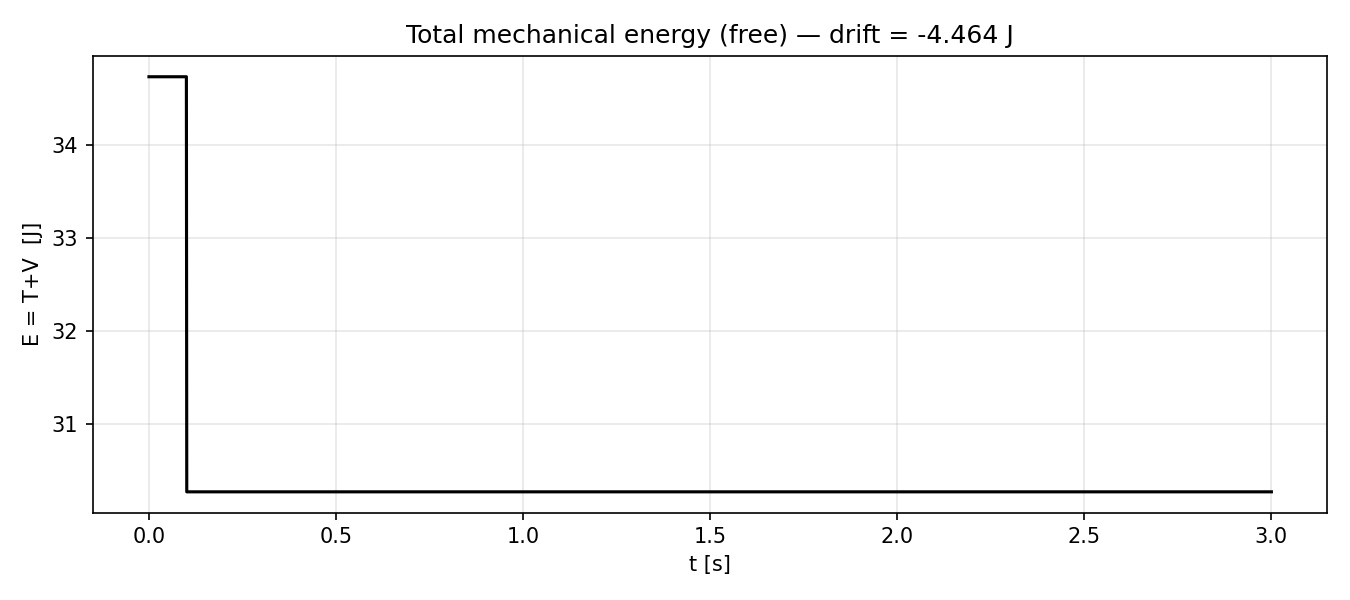
\includegraphics[width=0.62\textwidth]{../results/energy_free.png}
    \caption{שימור אנרגיה כוללת במצב תגובה חופשית ($\tau=0$). הסחיפה הנומרית קטנה מ-$10^{-6}$ ג'אול — מאמת את יציבות אינטגרטור ה-\textenglish{RK4} ואת דיוק מטריצות הדינמיקה.}
    \label{fig:energy_free}
\end{figure}

\begin{figure}[h]
    \centering
    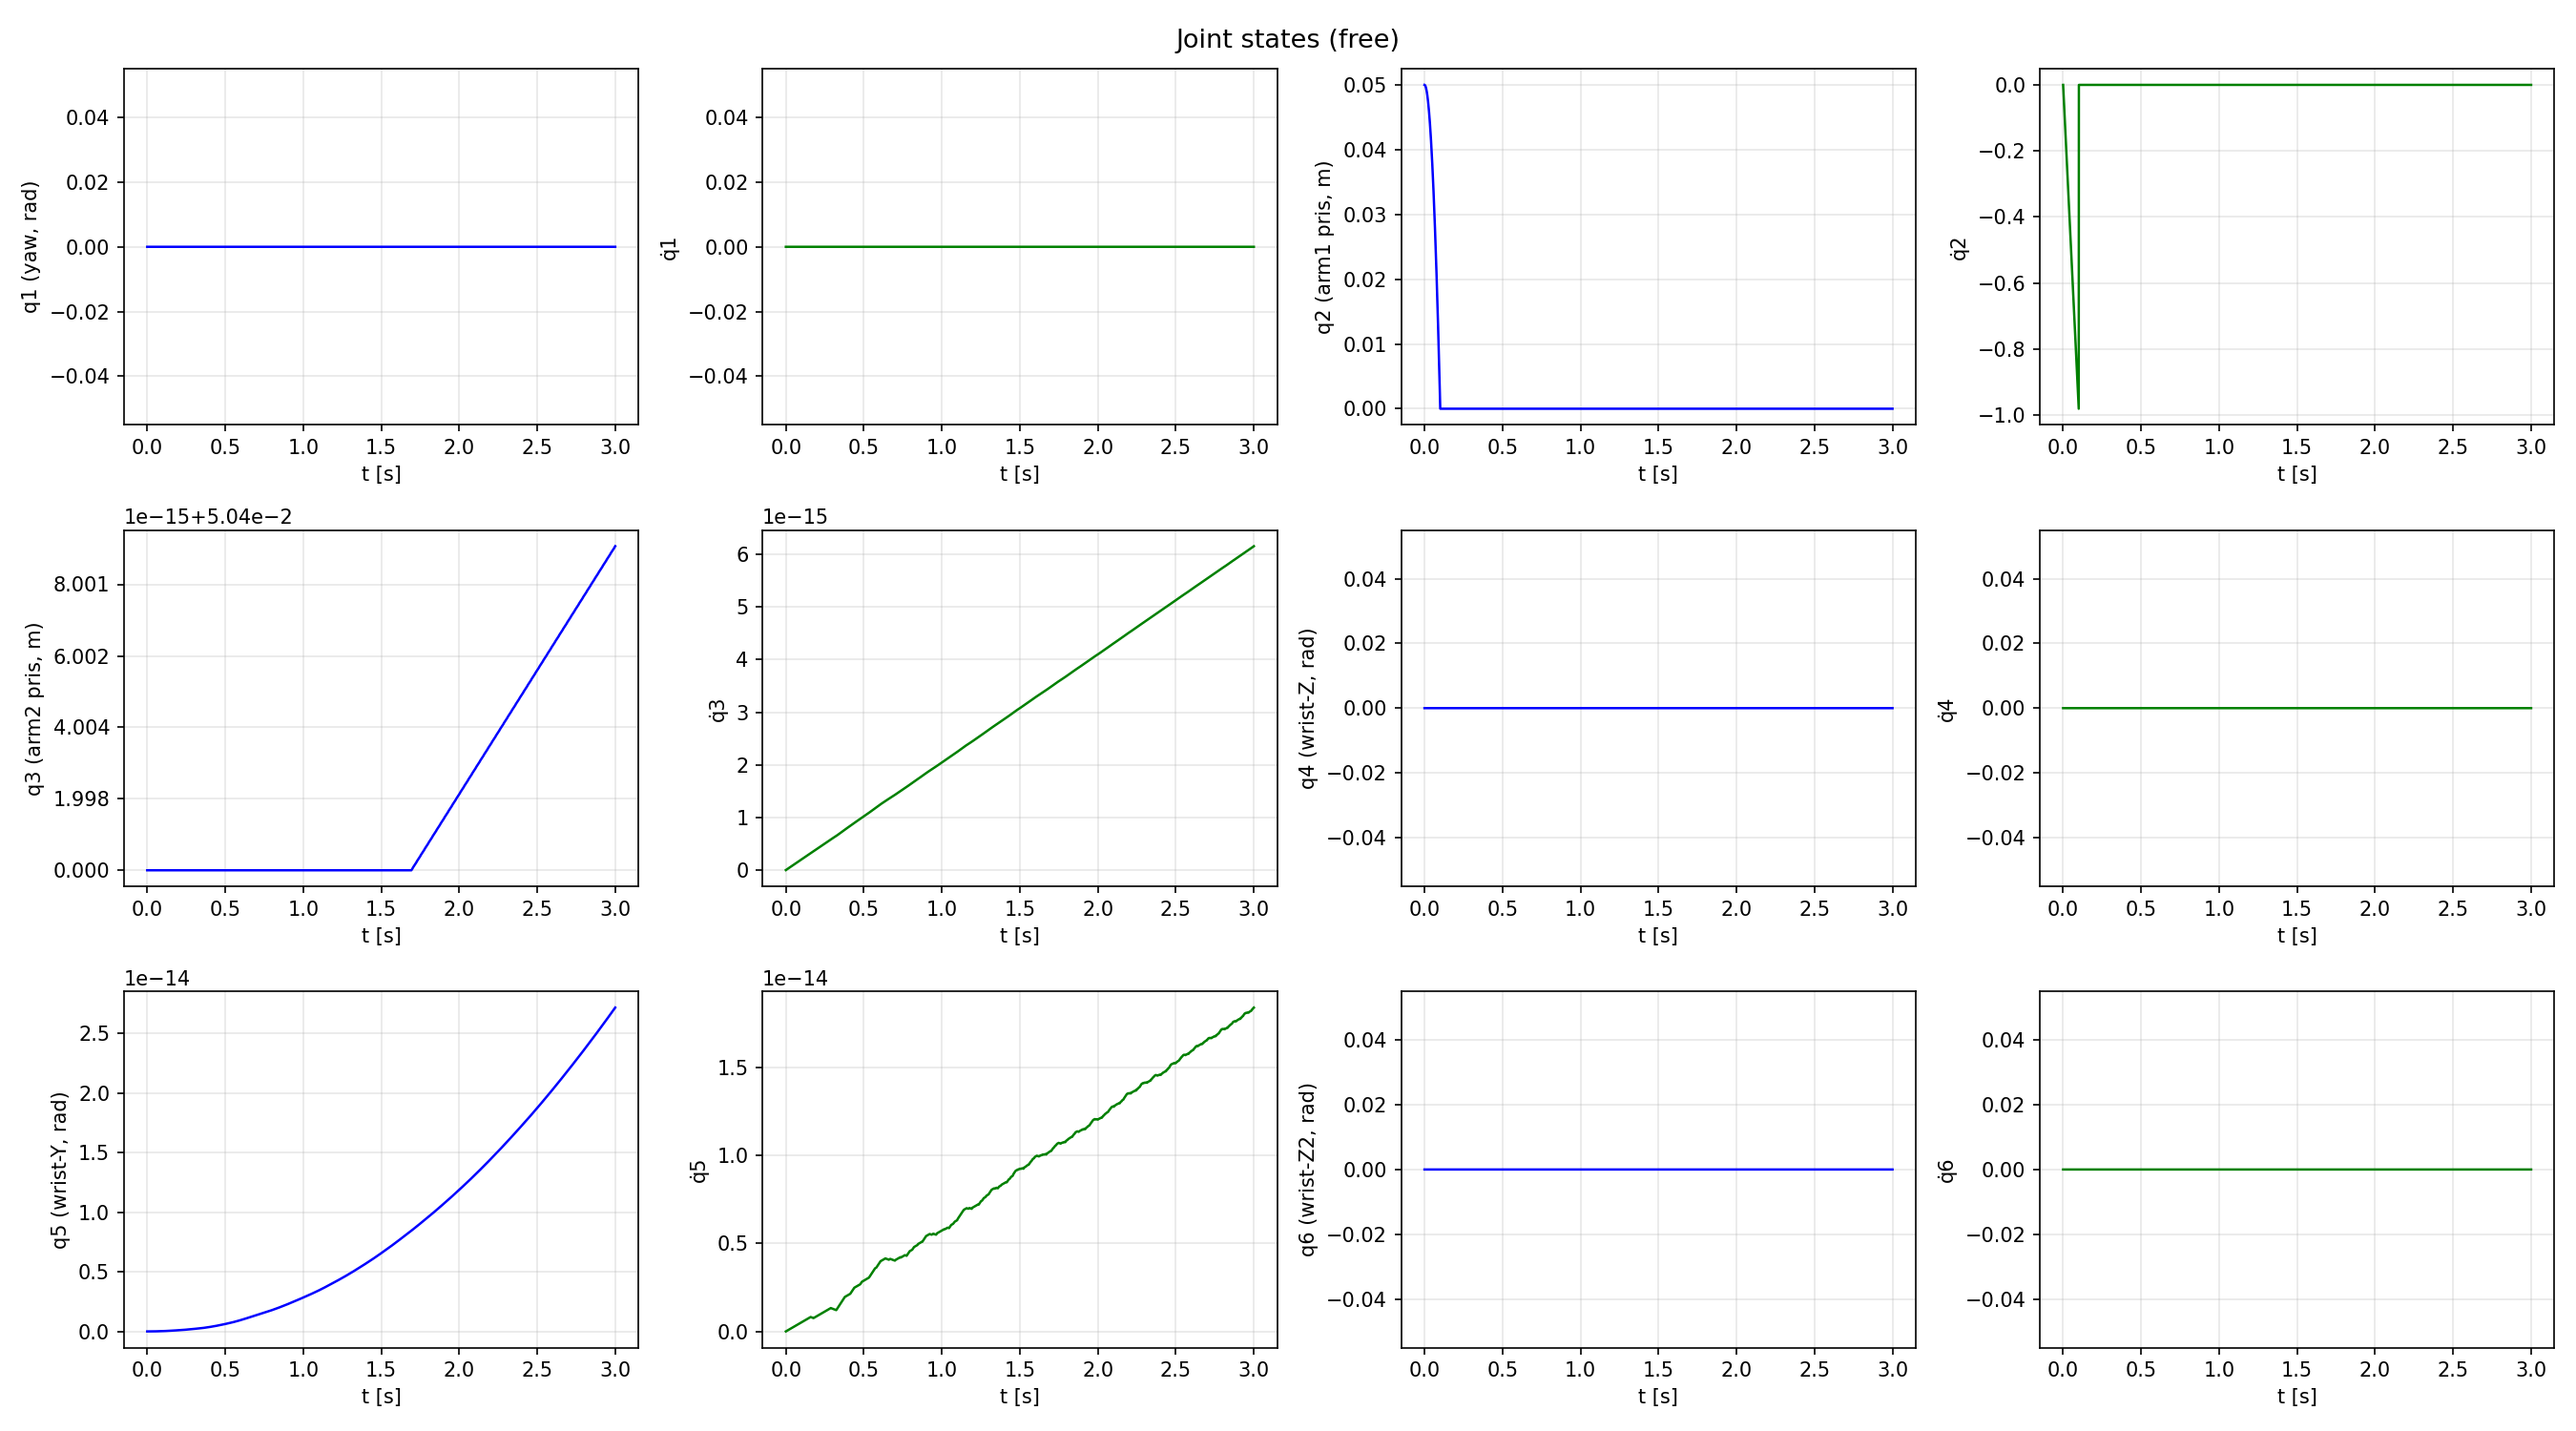
\includegraphics[width=0.80\textwidth]{../results/joint_states_free.png}
    \caption{גרפי פרמטרי הקונפיגורציה כפונקציה של זמן במצב תגובה חופשית ($\tau=0$). ניתן לראות את תנועת הרובוט תחת כוח הכובד בלבד — מפרקים פריזמטיים ($d_1, d_2$) שוקעים בהדרגה, ומפרקים סובבים ($\theta_1, \theta_4, \theta_5, \theta_6$) מתנודדים סביב שיווי המשקל.}
    \label{fig:joint_states_free}
\end{figure}

\begin{figure}[h]
    \centering
    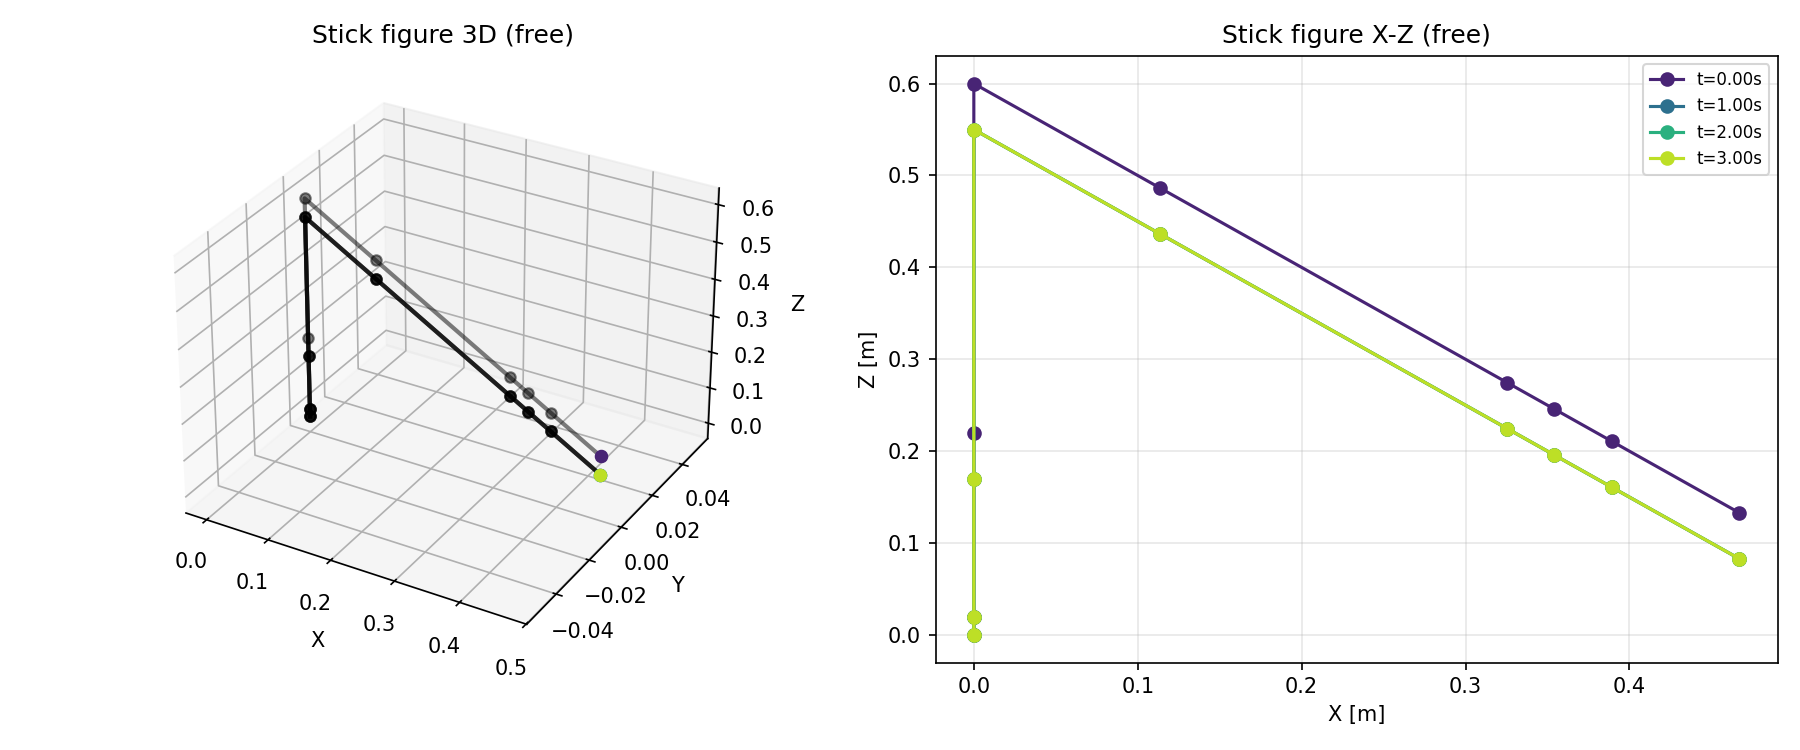
\includegraphics[width=0.75\textwidth]{../results/stick_snapshots_free.png}
    \caption{ייצוג \textenglish{Stick-Figure} בחתכי זמן עוקבים במצב תגובה חופשית ($\tau=0$). כל מסגרת מציגה את תצורת הרובוט בנקודת זמן שונה, המאפשרת בחינה ויזואלית של התנועה תחת כובד.}
    \label{fig:stick_free}
\end{figure}

\begin{figure}[h]
    \centering
    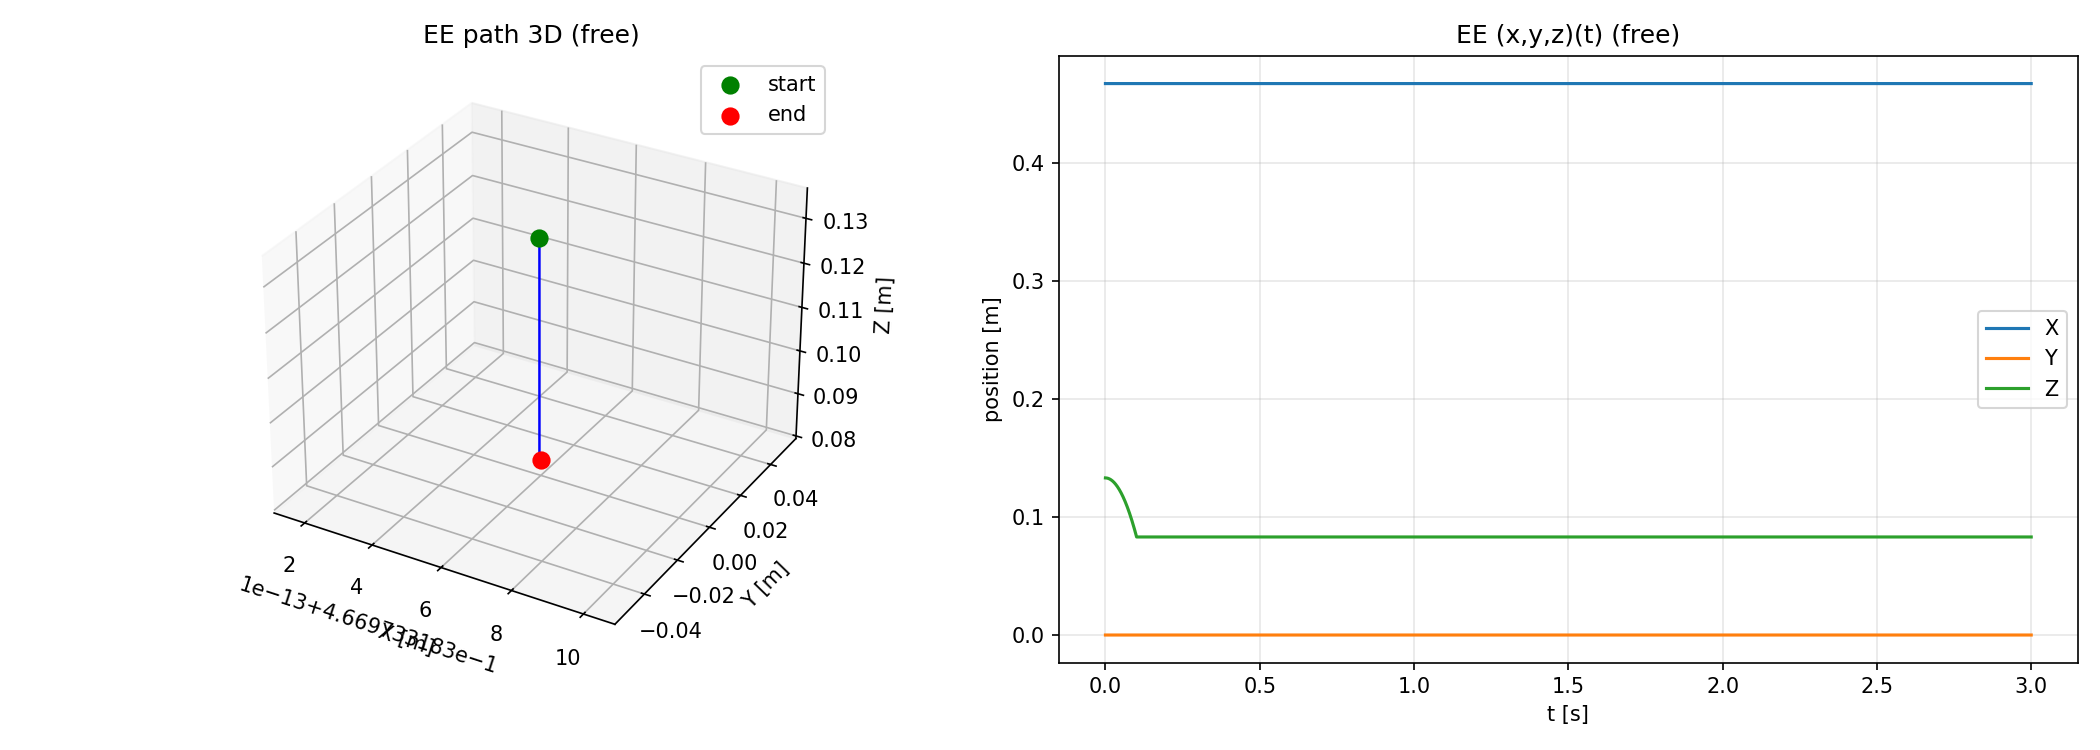
\includegraphics[width=0.60\textwidth]{../results/ee_path_free.png}
    \caption{מסלול קצה-האיבר (\textenglish{End-Effector}) במרחב המשימה במצב תגובה חופשית. הנתיב המרחבי של ה-\textenglish{EE} מתחיל בנקודת ההתחלה A ונע בהשפעת הכובד — ניתן לראות שאין כוח חיצוני המכוון אותו לנקודת היעד B.}
    \label{fig:ee_path_free}
\end{figure}


\section{תכנון בקר מבוסס-מודל (\textenglish{Computed-Torque PID})}
הרובוט מציג צימוד חזק בין המפרקים ולכן יושמה ארכיטקטורת \textenglish{Computed-Torque Control (CTC)} משולבת \textenglish{PID}.

\subsection{חוק הבקרה ודינמיקת השגיאה}
\begin{equation}
\tau = M(q)\underbrace{(\ddot{q}_d + K_d \dot{e} + K_p e + K_i \int e)}_{v} + C(q,\dot{q})\dot{q} + G(q)
\end{equation}
ניתן להבין מדוע חוק זה מבטל את הדינמיקה הלא-ליניארית על ידי הצבתו חזרה במשוואת התנועה~\eqref{eq:eom}:
\begin{align}
M(q)\ddot{q} + C(q,\dot{q})\dot{q} + G(q) &= M(q)v + C(q,\dot{q})\dot{q} + G(q) \nonumber \\
\implies \quad M(q)\ddot{q} &= M(q)v \nonumber \\
\implies \quad \ddot{q} &= v = \ddot{q}_d + K_d\dot{e} + K_p e + K_i\int e
\end{align}
מאחר ש-$e = q_d - q$ ולכן $\ddot{e} = \ddot{q}_d - \ddot{q}$, מתקבלת דינמיקת שגיאה לינארית ומפוצלת לפי מפרקים:
\begin{equation}
\ddot{e} + K_d \dot{e} + K_p e + K_i \int e = 0
\end{equation}
מכאן שהבקר "מבטל" את $M$, $C$ ו-$G$ בצד שמאל ומשאיר רק מערכת לינארית שאת התגובה שלה ניתן לעצב ישירות על ידי בחירת $K_p, K_d, K_i$ — זהו היתרון המרכזי של שיטת \textenglish{CTC} על פני \textenglish{PID} רגיל. כלומר, חוק \textenglish{CTC} מבצע ביטול משוב מדויק של כל האינרציות הלא-לינאריות (כולל אפקטי קוריוליס, תרומות צנטריפוגליות ועומסי כובד), ומייצר דינמיקת שגיאה לינארית ויציבה לחלוטין: הפולינום האופייני $s^2 + K_d s + K_p = 0$ מקנה ריסון קריטי ($\zeta = 1$) ומבטיח $e(t) \to 0$ באופן אקספוננציאלי עבור כל מפרק, ללא תלות בתצורת הרובוט.

\subsection{כיול הבקר ומניעת רוויה}
לריסון קריטי ($\zeta=1$), הגברי הבקר הוגדרו לפי $K_p = \omega_n^2$ ו-$K_d = 2\zeta\omega_n = 2\omega_n$, כאשר התדרים הטבעיים לכל מפרק הם $\omega_n = [5, 4, 4, 6, 6, 6]$ ראד/שנייה. ההגברים הנבחרים הם:
\begin{align*}
K_p &= [25.0,\ 16.0,\ 16.0,\ 36.0,\ 36.0,\ 36.0] \\
K_d &= [10.0,\ 8.0,\ 8.0,\ 12.0,\ 12.0,\ 12.0] \\
K_i &= [0.5,\ 0.5,\ 0.5,\ 0.5,\ 0.5,\ 0.5]
\end{align*}
הגבר $K_i$ קטן מסלק שגיאות מצב מתמיד הנובעות מחוסר התאמה מושלם של המודל. בנוסף, הוגדר מנגנון \textenglish{Anti-Windup} המגביל את מצבר האינטגרטור לתחום $\pm 5.0$ [rad/m] בכל מפרק, למניעת הצטברות שגיאה ולשמירה על היציבות.

\subsection{תוצאות תנועה בחוג סגור}
\begin{figure}[h]
    \centering
    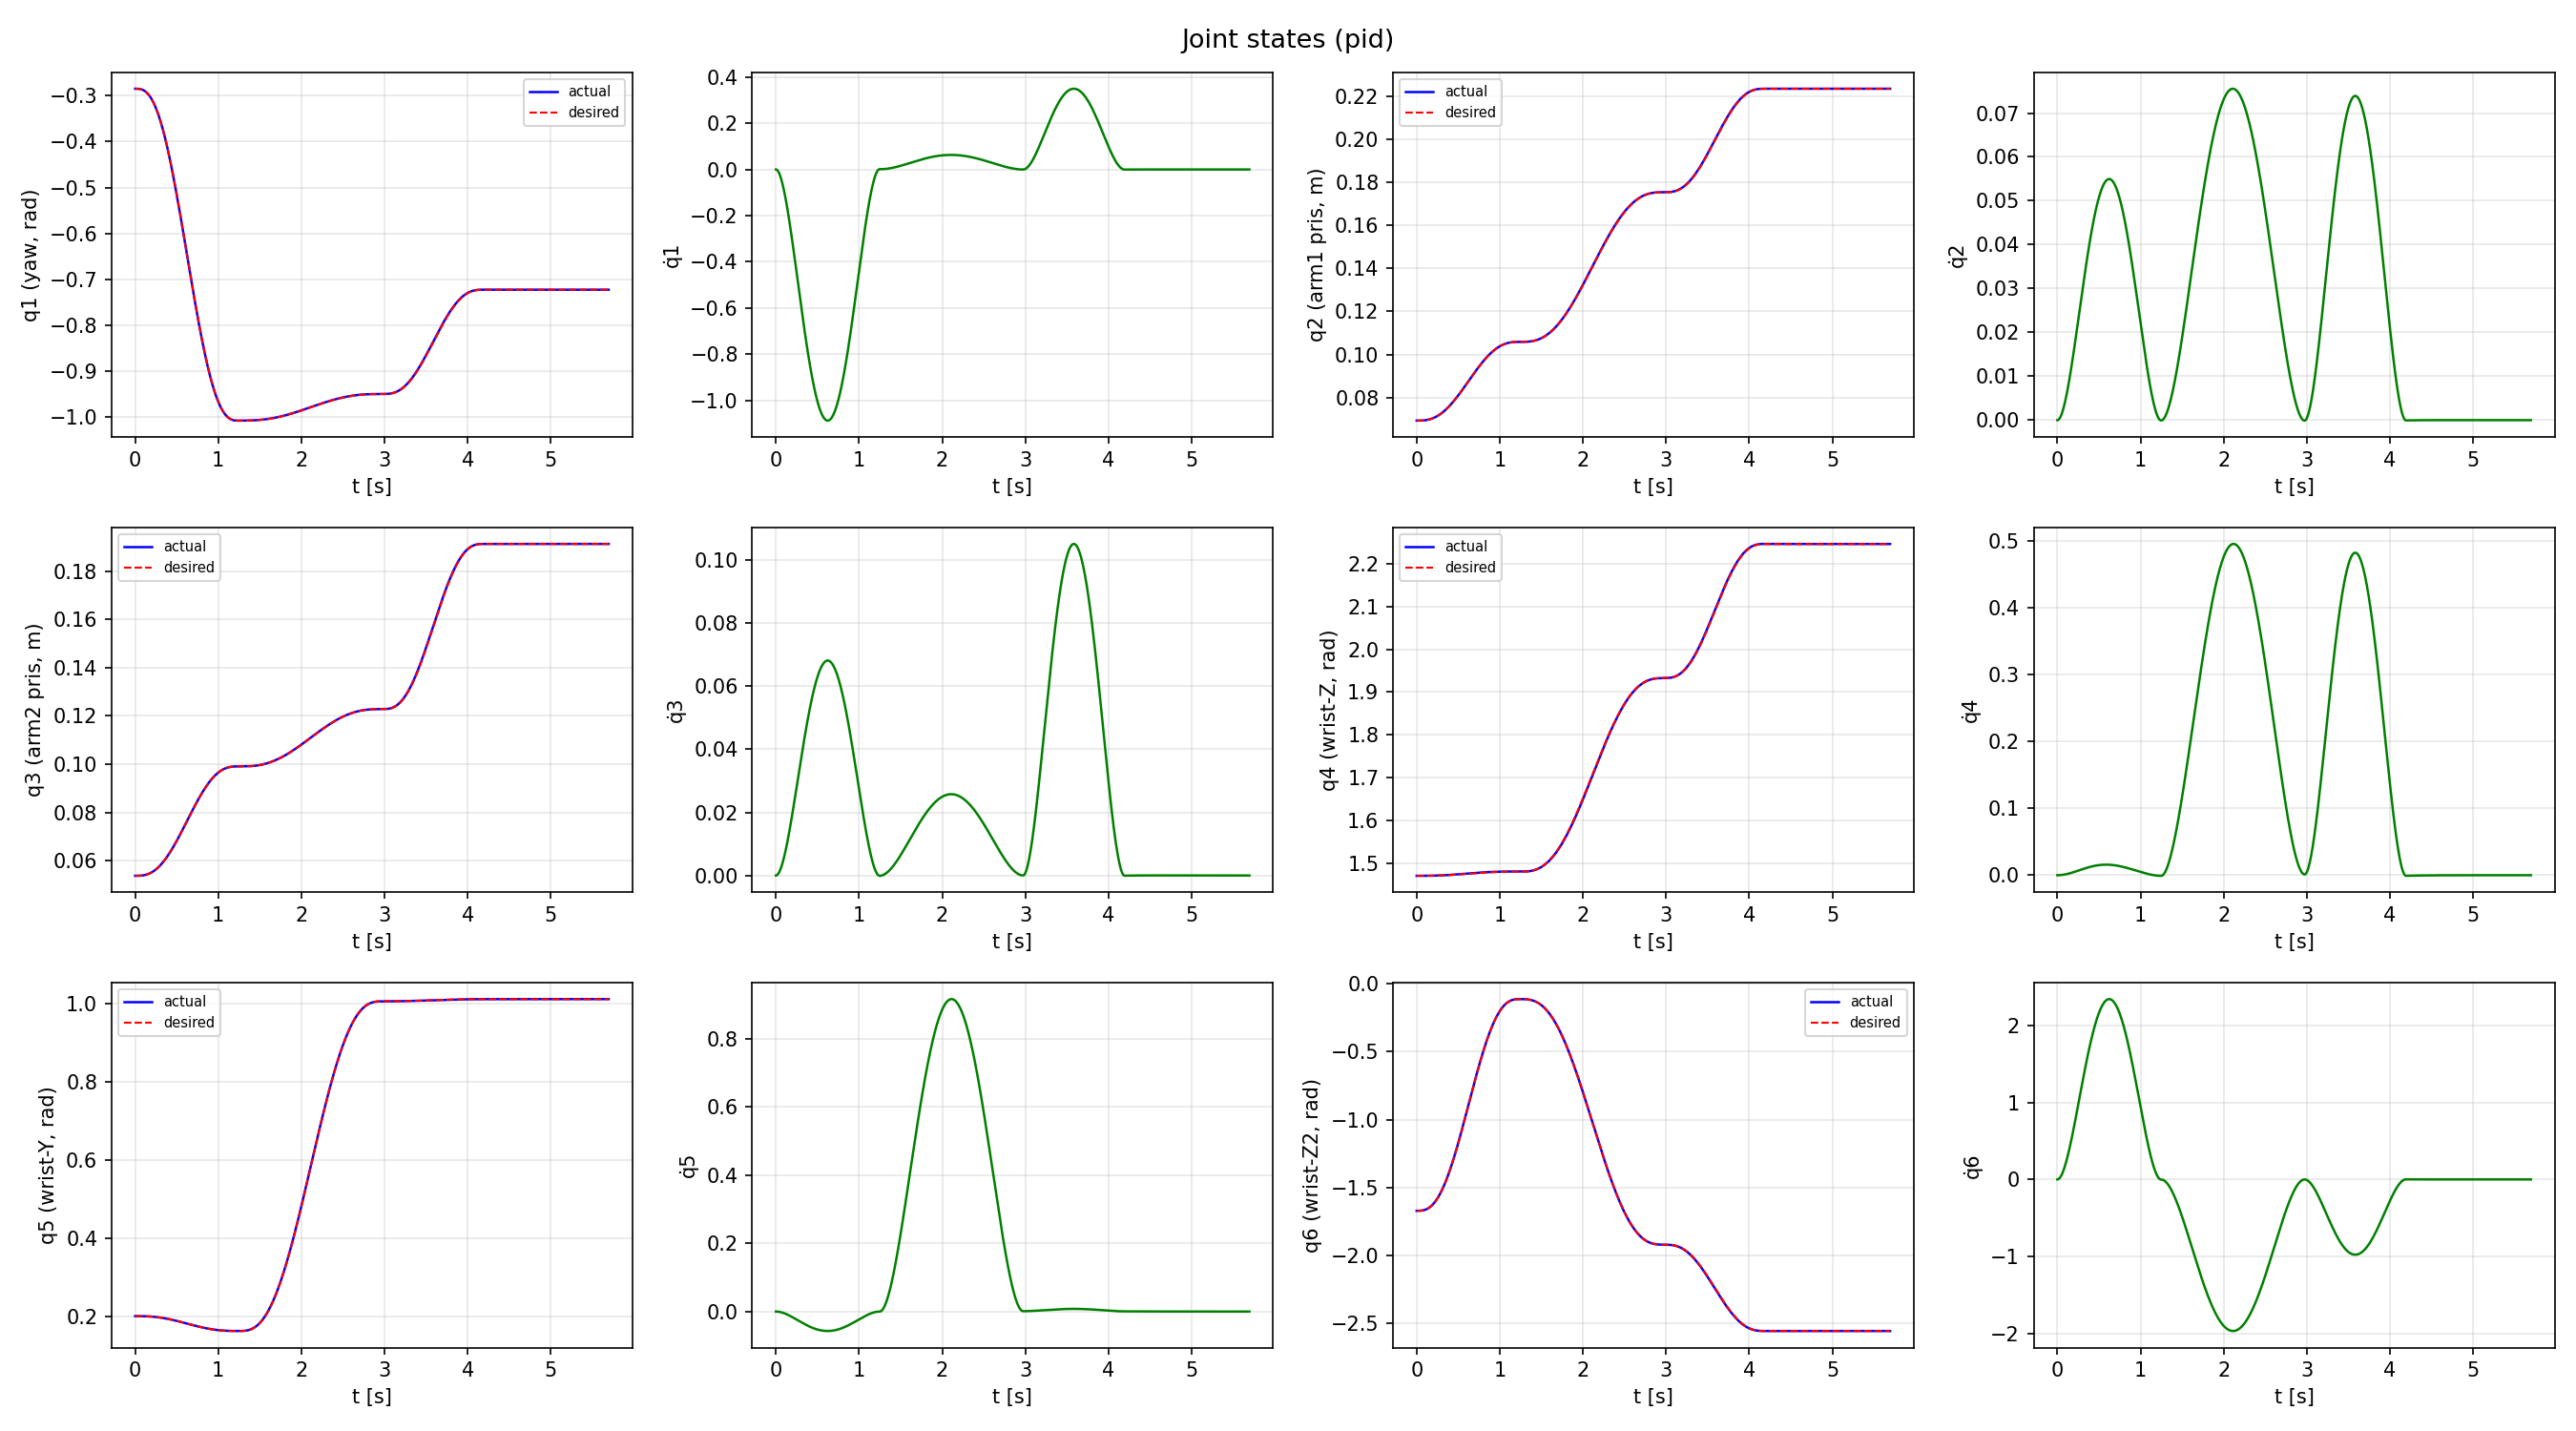
\includegraphics[width=0.7\textwidth]{../results/joint_states_pid.png}
    \caption{עקיבה אחר קונפיגורציית המפרקים לאורך זמן.}
    \label{fig:joint_states_pid}
\end{figure}

\begin{figure}[h]
    \centering
    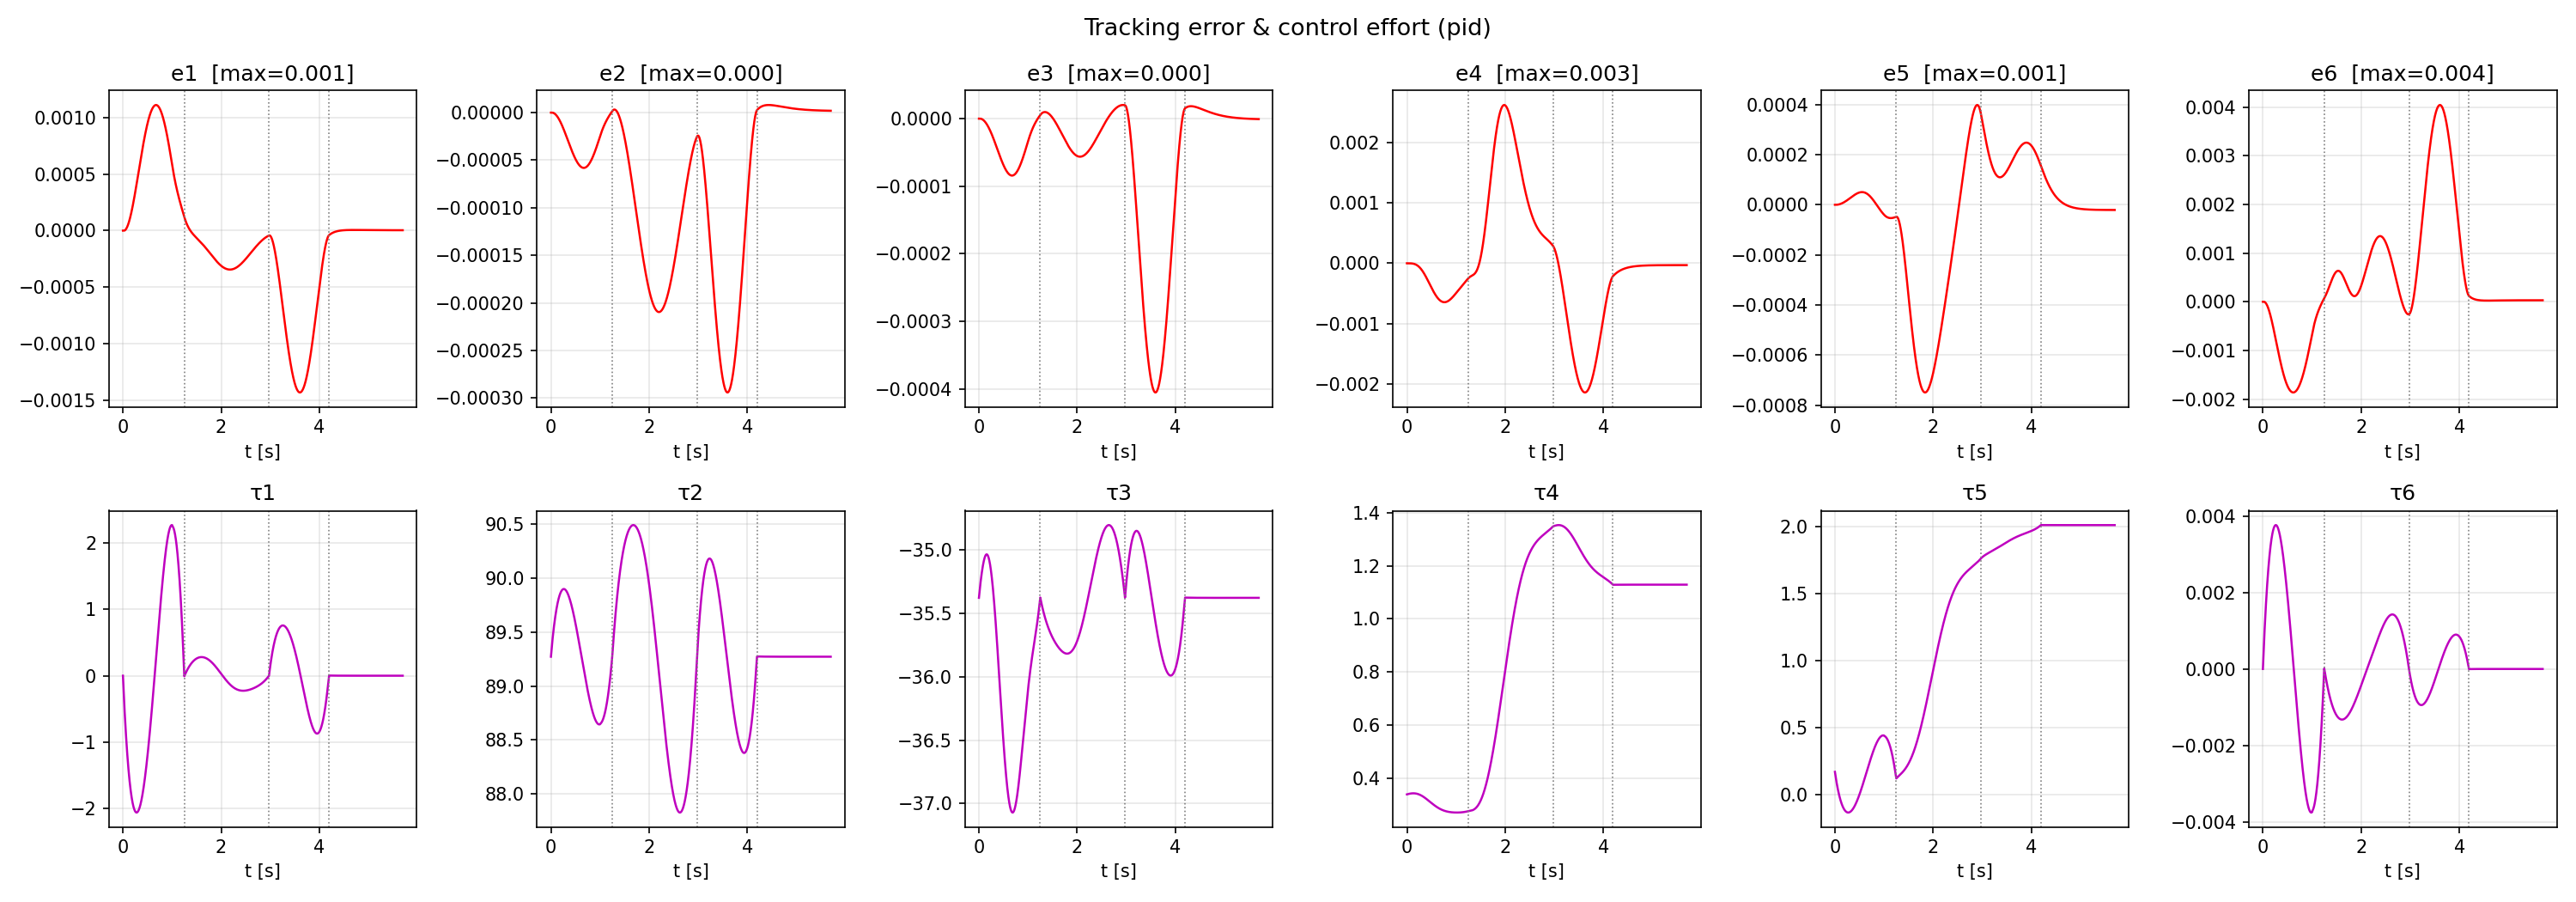
\includegraphics[width=0.7\textwidth]{../results/tracking_error_pid.png}
    \caption{שגיאת העקיבה ומומנטי המנועים.}
    \label{fig:tracking_error_pid}
\end{figure}

\begin{figure}[h]
    \centering
    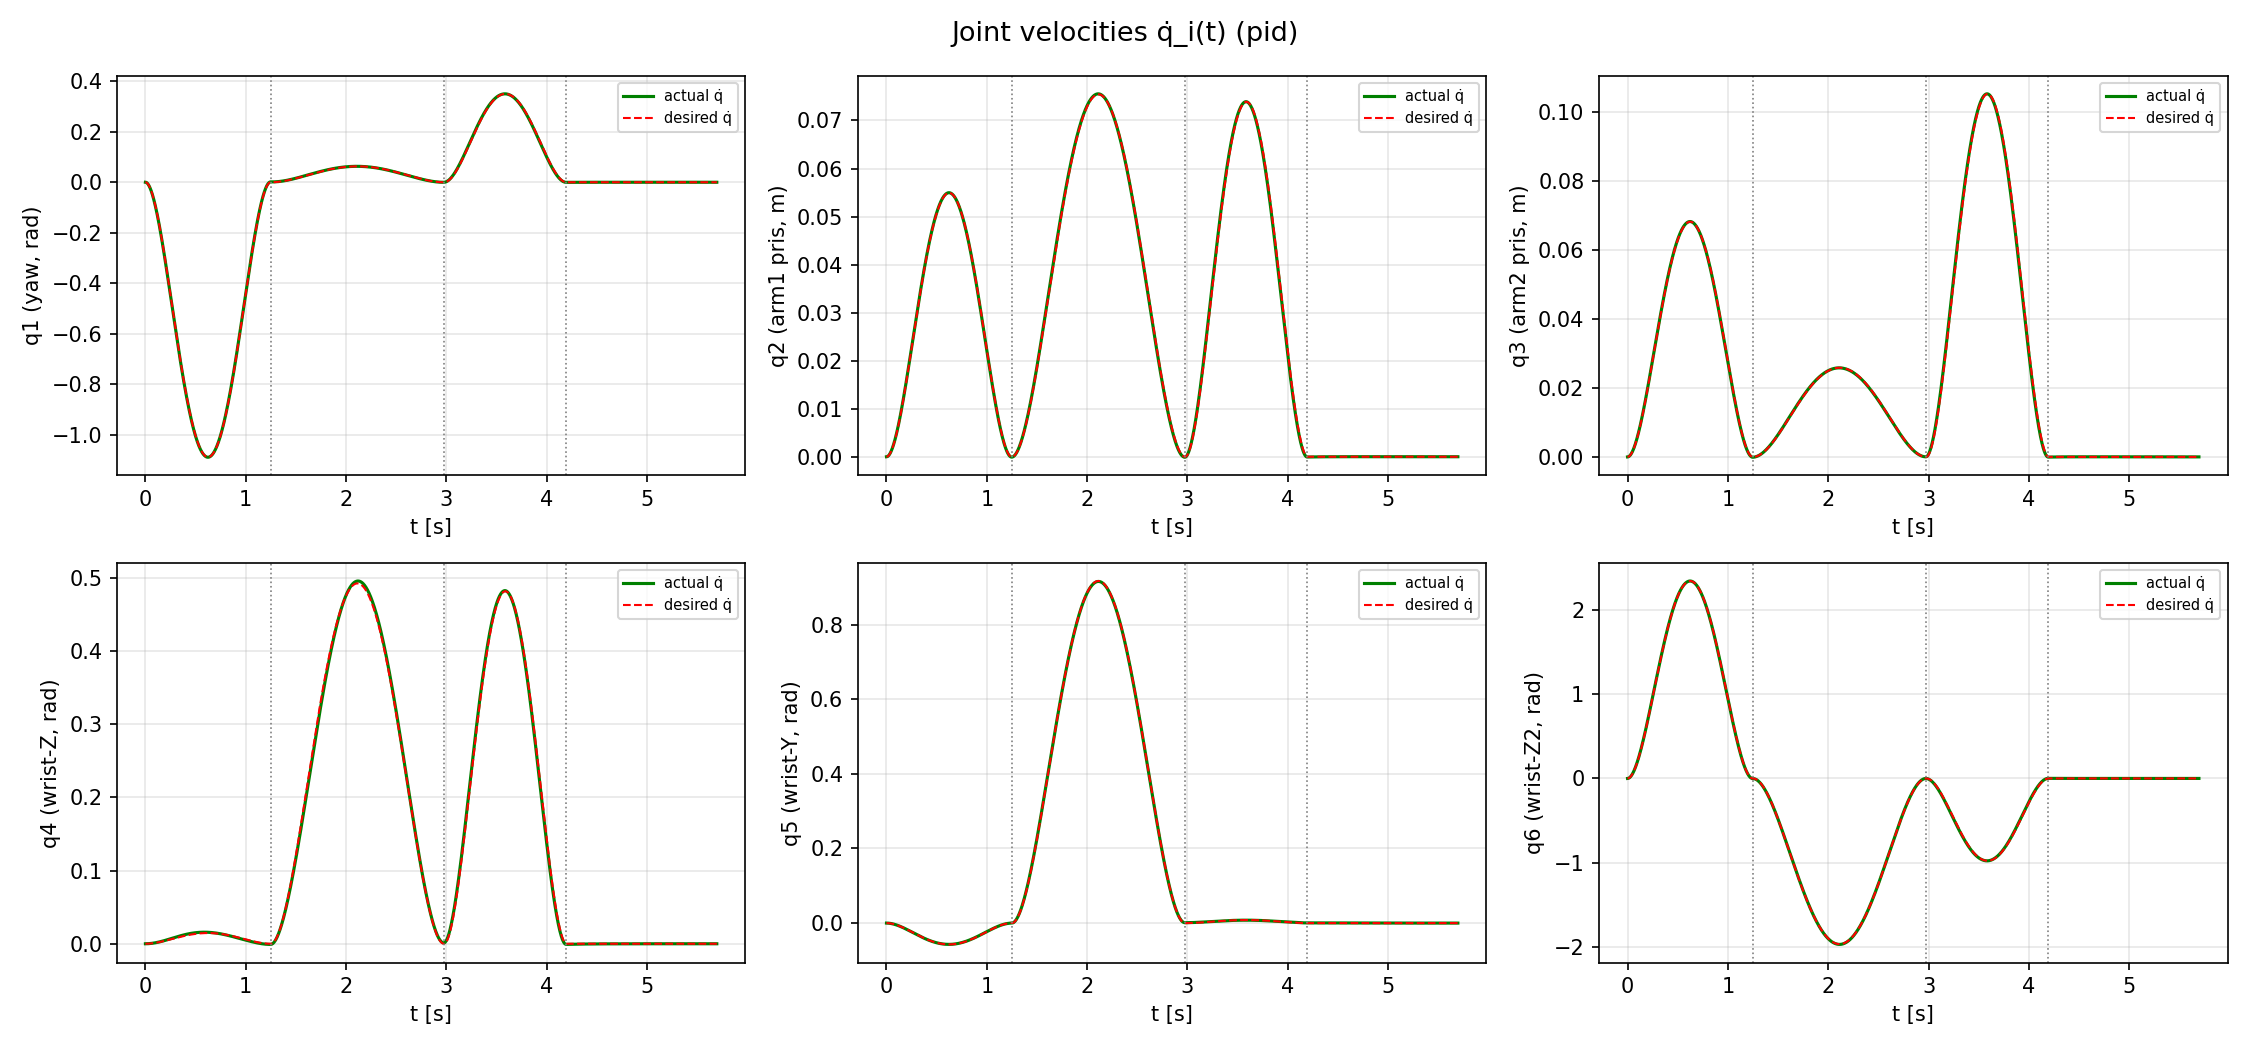
\includegraphics[width=0.7\textwidth]{../results/velocities_pid.png}
    \caption{פרופיל המהירויות לאורך המסלול.}
    \label{fig:velocities_pid}
\end{figure}

\begin{figure}[h]
    \centering
    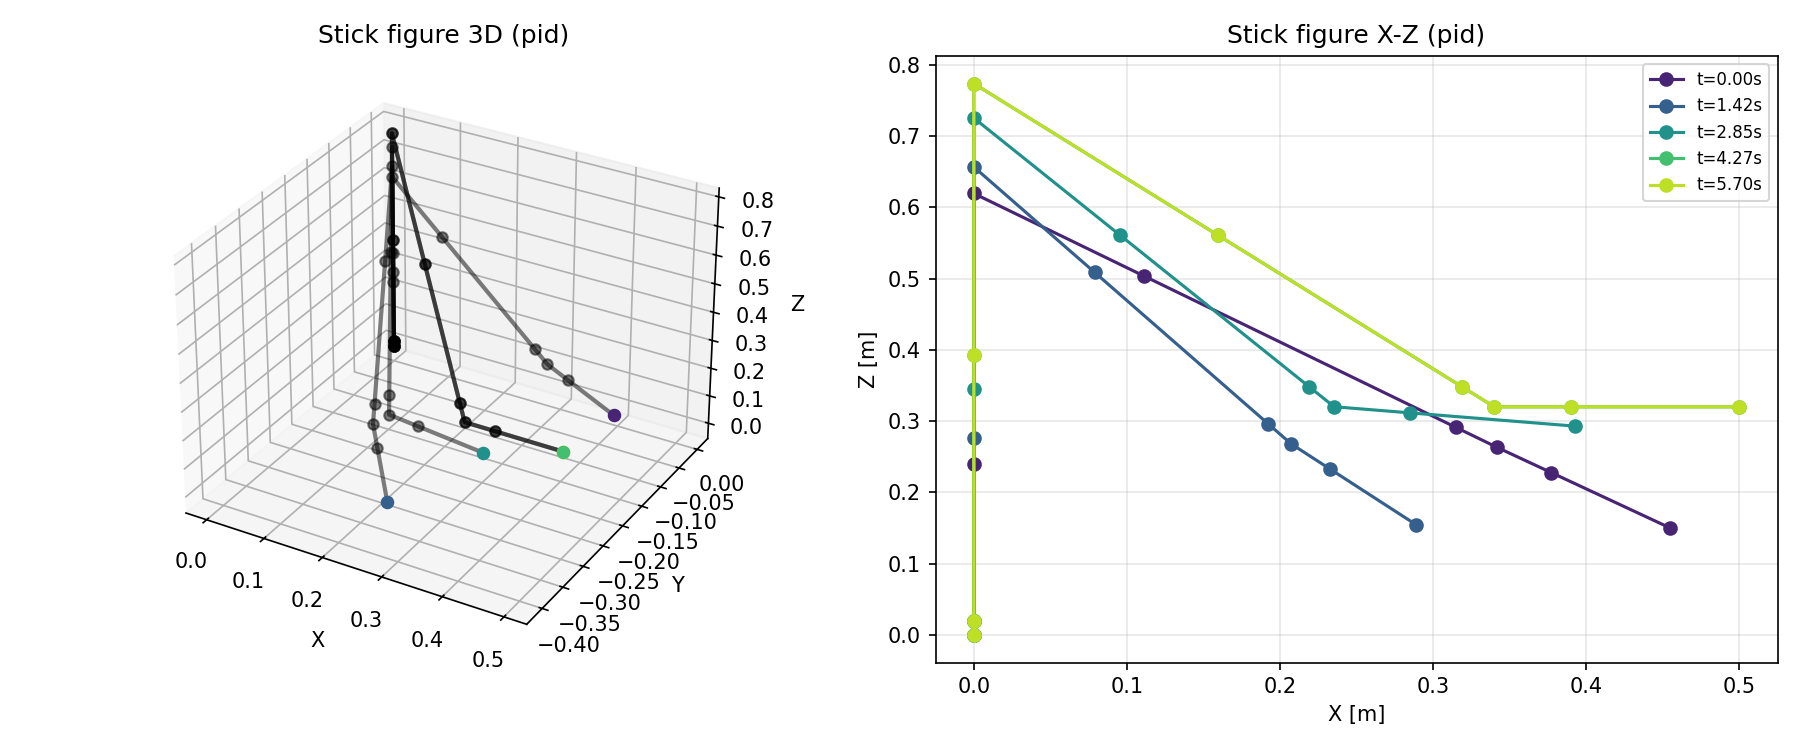
\includegraphics[width=0.7\textwidth]{../results/stick_snapshots_pid.png}
    \caption{חתכי זמן עוקבים של ייצוג ה-\textenglish{Stick-Figure} במהלך תנועת הרובוט תחת בקר ה-\textenglish{CTC+PID}. ניתן לראות את הרצף החלק של התנועה מנקודה A לנקודה B.}
    \label{fig:stick_snapshots_pid}
\end{figure}

\begin{figure}[h]
    \centering
    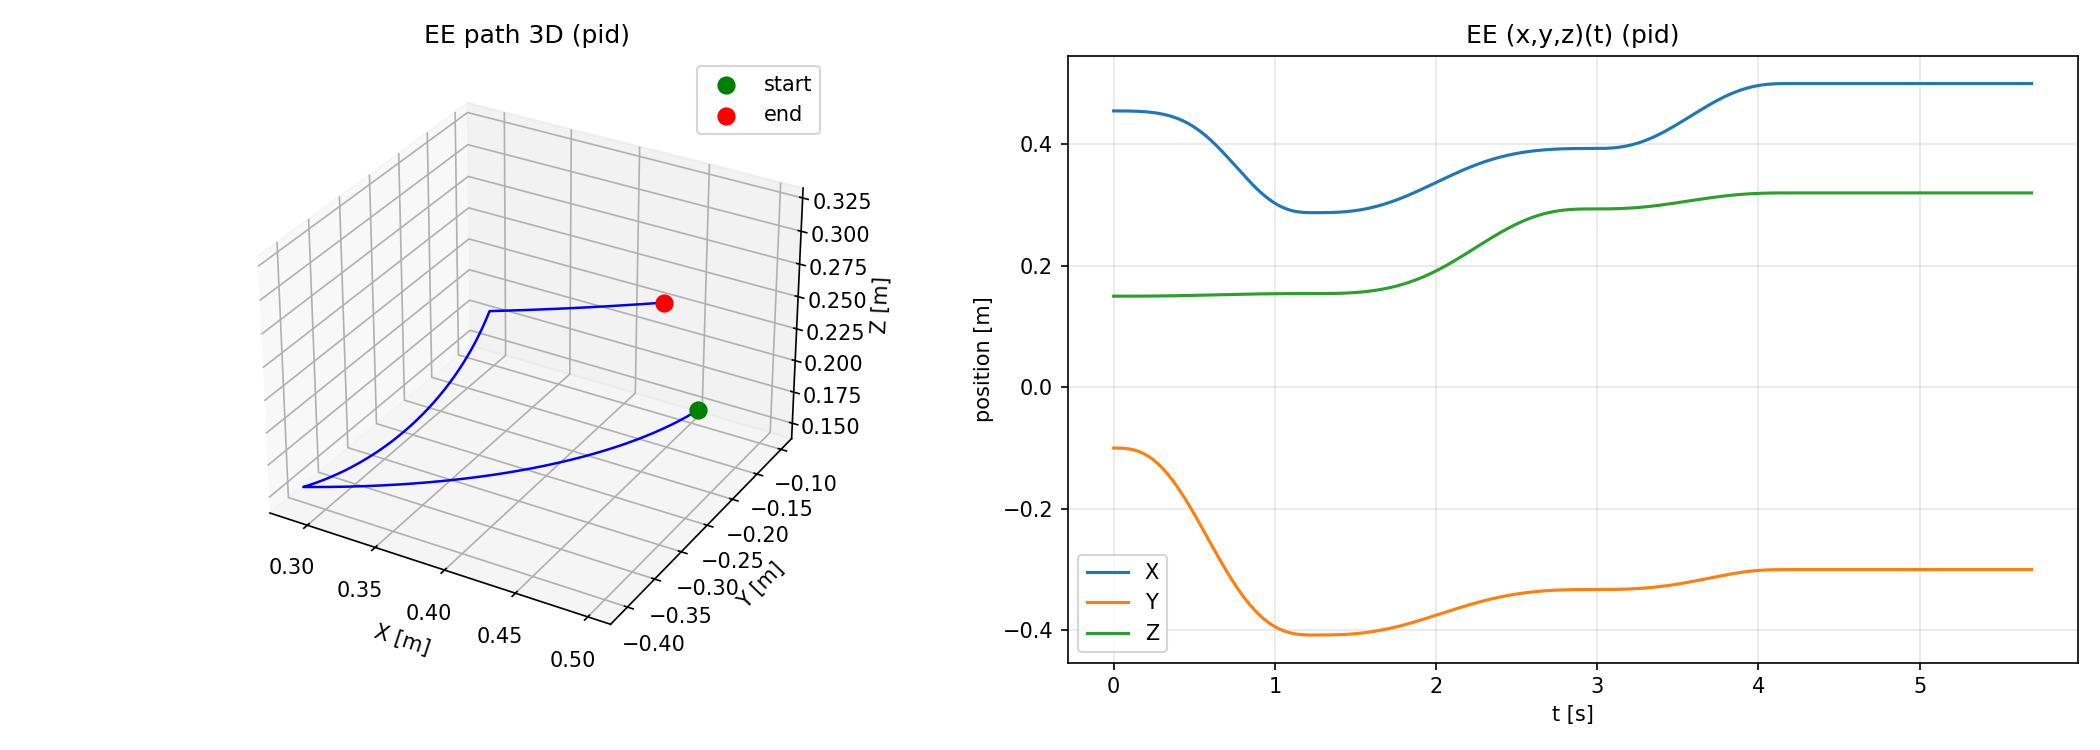
\includegraphics[width=0.60\textwidth]{../results/ee_path_pid.png}
    \caption{מסלול קצה-האיבר (\textenglish{End-Effector}) במרחב המשימה תחת בקר ה-\textenglish{CTC+PID}. הנתיב המרחבי עובר מנקודת ההתחלה A $(0.455, -0.1, 0.15)$ לנקודת היעד B $(0.50, -0.30, 0.32)$ תוך הימנעות מהתנגשות עם חציצת המדף.}
    \label{fig:ee_path_pid}
\end{figure}


\section{תכנון תנועה חופשי מהתנגשויות (\textenglish{Motion Planning \& Obstacle Avoidance})}
\subsection{מסלול פולינומי ממעלה חמישית (\textenglish{Quintic Polynomial Trajectory})}
לאחר שנקבעות נקודות הדרך ($q_0, q_f$) לכל קטע, נוצר מסלול רציף בעל תאוצה אפסית בקצוות (מינימום-ג'רק) באמצעות פולינום מסדר 5:
\begin{equation}
s(t) = a_3 t^3 + a_4 t^4 + a_5 t^5, \quad
a_3 = \frac{10}{T^3},\; a_4 = \frac{-15}{T^4},\; a_5 = \frac{6}{T^5}
\end{equation}
כאשר $q_d(t) = q_0 + s(t)(q_f - q_0)$, ו-$s(T)=1,\, \dot s(0)=\dot s(T)=\ddot s(0)=\ddot s(T)=0$.
מסלול זה מספק גם $\dot q_d$ וגם $\ddot q_d$ לבקר ה-\textenglish{CTC} ומבטיח יציאה ועצירה חלקות ללא בלימה פתאומית.

\subsection{מידול גיאומטרי ותכנון גלובלי}

\textbf{מדוע לתכנן ב-\textenglish{C-Space}?} \\
מרחב הקונפיגורציה (\textenglish{C-Space}) הוא מרחב שישה-ממדי שבו כל ציר מייצג מפרק אחד. כל נקודה בו מתארת קונפיגורציה מלאה של הרובוט. תכנון ישירות בו עדיף על תכנון במרחב המשימה, משום שבדיקת ההתנגשות מתבצעת פעם אחת לכל קונפיגורציה, ומשפחות של קונפיגורציות בטוחות ($Q_{free}$) מוגדרות מראש. יתרון נוסף: קיומם של פתרונות IK מרובים אינו מסבך את התכנון.

\textbf{מודל הקפסולות:} כל חוליה מיוצגת כגליל (קפסולה) ברדיוס $r = 35\,\text{mm}$. בדיקת התנגשות מחשבת את המרחק המינימלי מקטע הציר של הגליל לכל AABB של מכשול. קונפיגורציה חופשית מוגדרת כך: $\text{clearance}(q) > r + \text{margin}$, כאשר $\text{margin} = 10\,\text{mm}$ (סף סה"כ: 45 מ"מ).

\textbf{אלגוריתם \textenglish{biRRT} (DoubleTree RRT):} \\
בניגוד ל-\textenglish{RRT} הפשוט שבונה עץ אחד ממצב ההתחלה, \textenglish{biRRT} בונה שני עצים בו-זמנית — עץ $\mathcal{T}_A$ מ-$q_{start}$ ועץ $\mathcal{T}_B$ מ-$q_{goal}$ — ומנסה לחברם:
\begin{enumerate}
    \item \textenglish{EXTEND}($\mathcal{T}_A$, $q_{rand}$): נלקחת דגימה אקראית (או $q_{goal}$ בהסתברות של 20\%), נמצא הצומת הקרוב ביותר בעץ A, ומתבצעת הרחבה לעברה בצעד מנורמל.
    \item \textenglish{CONNECT}($\mathcal{T}_B$, $q_{new}$): מתבצע ניסיון לחבר את עץ B אל הצומת החדש בעץ A — חזרה על EXTEND לכיוון $q_{new}$ עד להגעה או לחסימה. כך גדל גם עץ B בכל ניסיון חיבור.
    \item עם חיבור מוצלח משורשר נתיב עץ A (התחלה$\rightarrow$פגישה) עם נתיב עץ B בסדר הפוך (פגישה$\rightarrow$יעד), והמסלול מקוצר באמצעות \textenglish{shortcutting} אקראי (400 ניסיונות).
\end{enumerate}
השיטה הדו-כיוונית (שני עצים עם מאמץ חיבור) מתכנסת מהר יותר מ-RRT חד-כיווני בסביבות צרות, שכן עץ B מצמצם את המרחק הנדרש לגישור.

\subsection{בדיקת מרווח בטיחות בזמן ריצה}
לאחר הסימולציה מתבצעת בדיקת מרווח: עבור כל נקודת זמן, נמדד המרחק המינימלי בין 8 נקודות הקפסולה לכל לוחות המדף. התנאי הנדרש הוא מרווח מינימלי של 3.6 ס"מ (סף המרווח שנקבע). הבדיקה מוכיחה כי ה-biRRT הבטיח הימנעות מהתנגשויות לאורך כל התנועה.

\begin{figure}[h]
    \centering
    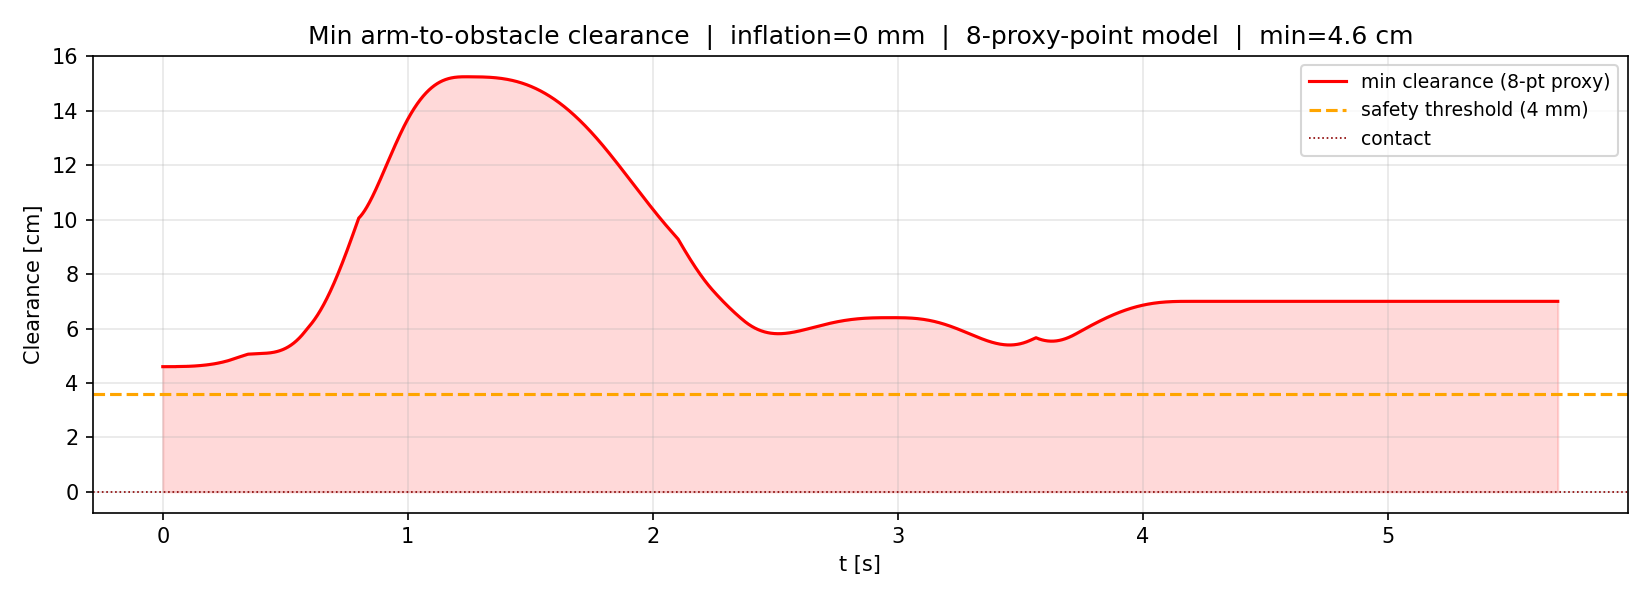
\includegraphics[width=0.7\textwidth]{../results/clearance_pid.png}
    \caption{מרווח בטיחות מינימלי מהמכשול לאורך הסימולציה — מעל לסף הנדרש (3.6 ס"מ).}
    \label{fig:clearance_pid}
\end{figure}


\section{מבנה התוכנה, סימולציה ב-\textenglish{Gazebo} ומסקנות}
\subsection{ארכיטקטורת התוכנה}
\begin{itemize}
    \item \texttt{\textenglish{urdf\_params.py}}: פרמטרים פיזיקליים ממקור האמת (ה-\textenglish{URDF}): מסות, מומנטי אינרציה, מגבלות מפרקים וקבועי הגיאומטריה.
    \item \texttt{\textenglish{kinematics.py}}: קינמטיקה ישירה ($^0T_8$) והפוכה (אנליטית + בחירת ענף) לחוליות מלאות.
    \item \texttt{\textenglish{dynamics.py}}: גזירה סימבולית של $M(q),C(q,\dot q),G(q)$ ב-\textenglish{SymPy}, שמירה למטמון וטעינה מחדש.
    \item \texttt{\textenglish{integrator.py}}: מימוש \textenglish{RK4} עצמאי, חישוב אנרגיה, וממשק \textenglish{SciPy RK45} לאימות.
    \item \texttt{\textenglish{controllers.py}}: בקר \textenglish{CTC+PID} עם \textenglish{Anti-Windup}, מחולל מסלול קווינטי (\textenglish{quintic polynomial}), ובסיסי השוואה: \textenglish{feedforward} בלבד ו-\textenglish{PID} טהור.
    \item \texttt{\textenglish{navigation.py}}: מודל הקפסולות (8 נקודות), מתכנן \textenglish{biRRT} ב-\textenglish{C-Space}, ובדיקת מרווח בטיחות.
    \item \texttt{\textenglish{simulate\_free.py}}: סימולציה ללא מומנטים לאימות שימור אנרגיה.
    \item \texttt{\textenglish{simulate\_pid.py}}: הרצת חוג הבקרה המלא (תכנון מסלול $\to$ \textenglish{CTC+PID} $\to$ ניווט $\to$ גרפים ו-\textenglish{CSV}).
    \item \texttt{\textenglish{gazebo\_control\_node.py}}: צומת \textenglish{ROS2} המשדר את המסלול מקובץ ה-\textenglish{CSV} לבקר ה-\textenglish{Gazebo} בזמן אמת.
\end{itemize}

\subsection{אינטגרציה עם \textenglish{ROS2} ו-\textenglish{Gazebo}}
{\sloppy המסלול המחושב ב-\textenglish{Python} מיוצא לקובץ \texttt{pid\_trajectory.csv}.
צומת \texttt{gazebo\_control\_node.py} קורא את הקובץ ומפרסם פקודות מיקום לכל אחד מ-6 המפרקים בתדר גבוה. הפקודות מגיעות לבקר המיקום \texttt{arm\_position\_controller}, בקר מסוג \textenglish{ForwardCommandController}, הפועל בתוך \textenglish{Gazebo}.
בכך משמש \textenglish{Gazebo} כפלטפורמת הדמיה ואימות של ה-\textenglish{URDF} ביחס לסימולציה הדינמית שבוצעה ב-\textenglish{Python}.\par}

\subsection{מסקנות}
הפרויקט מדגים בהצלחה תכנון, מודל מתמטי, ובקרת \textenglish{CTC} למניפולטור בן 6 דרגות חופש. להלן עיקרי הממצאים:

\begin{itemize}
    \item \textbf{אוילר-לגראנז':} גזירה סימבולית אוטומטית ב-\textenglish{SymPy} עם \textenglish{CSE} הצליחה לייצר קוד נומרי הרץ בזמן אמת, דבר שלא היה מעשי בגישה ידנית עבור שרשרת קינמטית מורכבת כזו.

    \item \textbf{CTC כ"ביטול דינמיקה":} הוכח שחוק הבקרה $\tau = M v + C\dot{q} + G$ הופך את הדינמיקה הלא-ליניארית של המניפולטור למערכת לינארית מפוצלת, מה שמאפשר כיול ישיר של הגברים לפי התדר הטבעי הרצוי לכל מפרק.

    \item \textbf{שכבות בקרה:} שילוב של שתי שכבות — תכנון גלובלי (\textenglish{biRRT}) ומסלול חלק (קווינטי) — הוכח כמספיק לסביבת המדף הנוכחית. התכנון הגלובלי מבטיח מסלול חף מהתנגשויות, והמסלול הקווינטי מבטיח שהבקר מקבל $\dot{q}_d$ ו-$\ddot{q}_d$ חלקים שמונעים בלימות פתאומיות.

    \item \textbf{אתגר המעבר הצר (\textenglish{Narrow Passage}):} מעבר הזרוע בין שני מדפים הצריך כוונון של מרווח הבטיחות המינימלי: ערך גדול מדי מונע ממצבי התחלה/יעד חוקיים להיחשב כ-$Q_{free}$, ערך קטן מדי מאפשר שגיאות מעקב שמובילות למגע בפועל.
\end{itemize}
% ==================== סוף חלק 1 ====================
\newpage

% ==================== תחילת חלק 2 ====================

\part{שיטת ניווט: \textenglish{FUEL} ורחפן אוטונומי}

\section{מבוא לחלק השני}

חלק זה מציג שיטת ניווט לחקר סביבה אוטונומי, המבוססת על המאמר
\textenglish{FUEL: Fast UAV Exploration using Incremental Frontier Structure and Hierarchical Planning}
(Zhou et al., IEEE RA-L, 2020).
השיטה משמשת כבסיס לתוכנת ניווט הרחפן שפותחה במסגרת פרויקט גמר העוסק בחיפוש בשטח באמצעות נחיל רחפנים אוטונומיים ב-\textenglish{ROS2/Gazebo}, בסביבה ללא מיפוי מוקדם וללא \textenglish{GNSS}.

\section{המאמר הנבחר — \textenglish{FUEL}}

\subsection{רקע ובעיה}

חקר אוטונומי (\textenglish{Autonomous Exploration}) הוא אחת המשימות הבסיסיות ביותר ברובוטיקה: כיצד ינווט רחפן לא-מאוייש (\textenglish{UAV}) בסביבה לא-ידועה, תוך כיסוי מרבי של השטח בזמן מינימלי ובבטחה? שיטות קלאסיות מבוססות \textenglish{frontier} (גבול החלל הנחקר) סובלות משתי מגבלות עיקריות:
\begin{itemize}
    \item חישוב מחדש של כל ה-\textenglish{frontiers} בכל שלב — עלות $O(N)$, כאשר $N$ מספר תאי המפה
    \item תכנון גלובלי מועט — הרחפן בוחר \textenglish{frontier} קרוב בלבד, ללא ראייה כוללת של המפה
\end{itemize}

\subsection{תרומות עיקריות}

המאמר מציג מסגרת היררכית בשלושה שלבים:
\begin{enumerate}
    \item \textbf{\textenglish{Frontier Information Structure (FIS)}}: מבנה נתונים המתוחזק באופן מצטבר (\textenglish{incremental}) והמתעדכן אך ורק באזורים שנסרקו מחדש, ללא סריקה מחדש של כל המפה. מאגר \textenglish{FIS} שומר לכל אשכול גבול: מיקום ממוצע, \textenglish{AABB}, נקודות תצפית אפשריות ועלויות קישוריות.

    \item \textbf{מתכנן גלובלי — סיור \textenglish{ATSP}}: בהינתן כל אשכולות ה-\textenglish{FIS} כתחנות, נפתרת בעיית ה-\textenglish{Asymmetric TSP} לתכנון מסלול ביקור גלובלי יעיל. כך הרחפן מכסה את כל אזורי הגבול ברצף אופטימלי, לא רק את הקרוב ביותר.

    \item \textbf{כיוון מקומי + מסלול \textenglish{B-spline}}: מתוצאת ה-\textenglish{ATSP} נבחר האשכול הבא; עבורו מתבצע חיפוש בגרף אחר נקודת תצפית מועדפת, ולבסוף מחושב מסלול \textenglish{B-spline} מינימום-זמן, ישים דינמית ובטוח.
\end{enumerate}

\subsection{ארכיטקטורה של \textenglish{FUEL}}

\begin{figure}[h]
    \centering
    \begin{minipage}{0.85\textwidth}
        \textbf{זרימת \textenglish{FUEL}:}\\[4pt]
        \textenglish{%
        Depth/Lidar sensor $\;\longrightarrow\;$ Incremental FIS update
        $\;\longrightarrow\;$ ATSP global tour
        $\;\longrightarrow\;$ Local viewpoint refinement
        $\;\longrightarrow\;$ Min-time B-spline trajectory
        $\;\longrightarrow\;$ UAV velocity commands}
    \end{minipage}
    \caption{תרשים זרימה של אלגוריתם \textenglish{FUEL}: עדכון מצטבר של ה-\textenglish{FIS}, תכנון גלובלי (\textenglish{ATSP}), כיוון מקומי ומסלול \textenglish{B-spline}.}
    \label{fig:fuel_pipeline}
\end{figure}

\subsection{תוצאות המאמר}

ב-\textenglish{benchmark} בסביבות סגורות מורכבות, \textenglish{FUEL} מגיע לכיסוי 90\% מהר פי 3-8 מהשיטות המובילות הקודמות (\textenglish{NBVP, GBPlanner, RACER}). עיקר השיפור נובע מ:
\begin{itemize}
    \item עדכון \textenglish{FIS} מצטבר — הופך את עלות העדכון מ-$O(N)$ ל-$O(\Delta N)$
    \item תכנון \textenglish{ATSP} גלובלי — מונע תנודות הלוך-ושוב בין גבולות סמוכים
    \item מסלול \textenglish{B-spline} בטוח — מאפשר מהירויות גבוהות יותר ביחס לשיטות שמורידות מהירות ליד מכשולים
\end{itemize}

\section{מבנה תוכנת פרויקט הרחפן ב-\textenglish{ROS2}}

\subsection{ארכיטקטורת החבילות}

הפרויקט מורכב מ-6 חבילות \textenglish{ROS2 (C++/Python)}, הפועלות עם \textenglish{PX4 SITL} ו-\textenglish{Gazebo Harmonic} בסביבה ללא \textenglish{GNSS}:

\begin{table}[H]
\centering
\begin{tabular}{cc}
\toprule
\textbf{חבילה} & \textbf{תפקיד} \\
\midrule
\textenglish{swarm\_sim\_bringup} & השקת \textenglish{Gazebo + PX4 SITL} וגשרי חיישנים (\textenglish{RGB-D, LiDAR, range}) \\
\textenglish{swarm\_perception} & \textenglish{voxel\_mapper}: מיפוי \textenglish{log-odds} תלת-ממדי, גילוי גבולות ותכנון \textenglish{A*} \\
\textenglish{swarm\_bringup} & בקר משימה (\textenglish{FSM + VFH}), היתוך מיקום \textenglish{SLAM+PX4}, משגר ראשי \\
\textenglish{swarm\_target\_detection} & זיהוי מטרות (\textenglish{HSV blob}) ממצלמת \textenglish{RGB-D} \\
\textenglish{swarm\_msgs} & הגדרות הודעות (\textenglish{messages}) מותאמות אישית \\
\textenglish{swarm\_coordination} & בסיס לתיאום עתידי בין רחפנים בנחיל \\
\bottomrule
\end{tabular}
\caption{חבילות ה-\textenglish{ROS2} בפרויקט הרחפן ותפקידן.}
\label{tab:ros2_packages}
\end{table}

\subsection{הצמתים הראשיים בסימולציית רחפן יחיד}

קובץ ההשקה \textenglish{d1\_single\_agent\_search.launch.py} מפעיל את הצמתים הבאים:

\begin{enumerate}
    \item \textbf{\textenglish{voxel\_mapper}} (\textenglish{swarm\_perception, C++}): לב המערכת. מקבל פריימי עומק מ-\textenglish{OAK-D Lite}, מבצע \textenglish{ray-casting} הסתברותי לתוך מפת וקסל תלת-ממדית (\textenglish{log-odds}, רזולוציה 0.2 מ'), מחשב שכבת 2D בגובה הרחפן, מזהה אשכולות גבול (\textenglish{FIS}), מתכנן נתיב \textenglish{A*} ומפרסם \textenglish{frontier\_path}.

    \item \textbf{\textenglish{search\_mission\_controller}} (\textenglish{swarm\_bringup, C++}): \textenglish{FSM} ראשי + בקר \textenglish{VFH} \textbf{הולונומי}. שולח פקודות מהירות $v_N, v_E$ ישירות (ללא תלות בכיוון האף), כאשר \textenglish{yaw} מנוהל בנפרד עם הגבלת קצב 30$^{\circ}$/ש'.

    \item \textbf{\textenglish{slam\_to\_px4}} (\textenglish{swarm\_bringup, Python}): סינון שער רב-שלבי — בודק קפיצות מרחביות ($>$0.75 מ'), סחיפת \textenglish{yaw} ($>$0.55 ראד) וקצב ה-\textenglish{yaw} של ה-\textenglish{SLAM} ($>$90$^{\circ}$/ש'). עם שער פעיל: \textenglish{PX4 EKF2} חוזר ל-\textenglish{IMU} בלבד (עד 750 מילישניות — drift $<$0.2$^{\circ}$). היסטרזיס: פעיל אחרי 2 פריימים רעים, מתנקה אחרי 15 טובים.

    \item \textbf{\textenglish{target\_detector}} (\textenglish{swarm\_target\_detection}): גילוי מטרות בצבע אדום על פי \textenglish{HSV blob detection} בפריים ה-\textenglish{RGB}.

    \textbf{הערה ארכיטקטורית}: חיישן \textenglish{LiDAR} 2D (\textenglish{RPLIDAR A2M8}) \textbf{הוסר לחלוטין} מהמערכת. כל המיפוי ה-3D מבוסס על מצלמת \textenglish{OAK-D Lite} בלבד. פרמטר \texttt{integrate\_lidar\_into\_map=false} ב-\textenglish{voxel\_mapper} מאשר זאת — הצומת אינו נרשם לנושא ה-\textenglish{LiDAR} כלל.
\end{enumerate}

\section{שיטת הניווט — שילוב \textenglish{FUEL Frontier} עם \textenglish{VFH} ותכנון \textenglish{A*}}

שיטת הניווט בנויה משלוש שכבות מקוננות, המבוססות על ארכיטקטורת ה-\textenglish{FUEL} תוך התאמה הנדסית מכוונת לאילוצי הרחפן:

\begin{table}[H]
\centering
\begin{tabular}{ccc}
\toprule
\textbf{שכבה} & \textbf{תפקיד} & \textbf{השראה מ-\textenglish{FUEL}} \\
\midrule
מיפוי + \textenglish{FIS} & גילוי גבולות מצטבר & ישיר ($O(\Delta N)$) \\
תכנון גלובלי & \textenglish{A*} עם עונש \textenglish{Voronoi} & אדפטציה של \textenglish{ATSP} \\
בקר מקומי & \textenglish{VFH} אוניציקלי & אדפטציה של \textenglish{B-spline} \\
\bottomrule
\end{tabular}
\caption{שלוש שכבות שיטת הניווט והשראתן מארכיטקטורת \textenglish{FUEL}.}
\label{tab:nav_layers}
\end{table}

\subsection{מודל קינמטי — \textenglish{VFH} הולונומי עם \textenglish{Yaw} מנותק}\label{sec:holonomic_model}

הרחפן פועל במצב \textenglish{Offboard} של \textenglish{PX4} ב\textbf{תצורה הולונומית} (\textenglish{Holonomic Mode}): \textenglish{TrajectorySetpoint} שולח מהירות ישירות בשני הצירים $v_N, v_E$ ללא תלות בכיוון האף, כאשר \textenglish{yaw} נשלט בנפרד:

\begin{equation}
v_N = v_{max}\cos\psi_{VFH}, \quad v_E = v_{max}\sin\psi_{VFH}, \quad \dot{\psi}_{cmd} = \text{slew}(\psi_{target} - \psi_{current},\; \dot{\psi}_{max})
\end{equation}

\textbf{מדוע תצורה הולונומית ולא אוניציקלית?} \\
הגרסה הקודמת של המערכת הפעילה \textenglish{Yaw-First Alignment}: הרחפן סובב לכיוון ה-VFH לפני כל תנועה. פרקטיקה זו גרמה לסחיפת SLAM חמורה — הסיבובים המהירים הכניסו רעש לקריאות החיישן ופגמו ביכולת ה-SLAM לעקוב אחר המיקום. \textbf{המעבר לתצורה ההולונומית פתר זאת}:
\begin{enumerate}
    \item כיוון ה-\textenglish{yaw} נשמר כמעט קבוע לכיוון היעד הנוכחי — ללא סיבובים מהירים.
    \item תנועה מבוצעת לכיוון שנבחר על ידי \textenglish{VFH} ישירות, גם אם שונה מכיוון האף.
    \item \textbf{עצירת בטיחות קדמית}: אם \texttt{forward\_range < 0.45m} וזווית האף לכיוון \textenglish{VFH} $> 0.30$ ראד — $v_N = v_E = 0$ (עצירת בטיחות).
\end{enumerate}

שינוי זה, בשילוב הסרת ה-\textenglish{LiDAR} והשבתת סריקת ההמראה, הביא לייצוב מלא של מערכת ה-\textenglish{SLAM} ולכיסוי שטח של 69.5\%.

\textbf{עקרון ה-\textenglish{PX4 TrajectorySetpoint} ב-velocity mode}:
\begin{itemize}
    \item \texttt{velocity = \{v\_N, v\_E, v\_Z\}} — מהירות NED ישירה
    \item \texttt{yaw = yaw\_abs} — כיוון מוחלט (ראד)
    \item \texttt{yawspeed = NaN} — מתעלם; yaw נשלט דרך השדה \texttt{yaw} בלבד
\end{itemize}

התאמה זו אף קרובה יותר להנחות ה-\textenglish{FUEL} המקורי (המניח \textenglish{holonomic agent}) מאשר הגרסה האוניציקלית — ה-\textenglish{PX4 X500} מסוגל לתנועה הולונומית מלאה.

\subsection{מיפוי תלת-ממדי — \textenglish{voxel\_mapper}}

הצומת \textenglish{voxel\_mapper} בונה מפת וקסל עולמית בתחום \textenglish{NED}: $N \in [-9, 9]$ מ', $E \in [-9, 31]$ מ', $Z \in [-11, 0.5]$ מ' (18,000 תאים בשכבה ברזולוציה 0.2 מ'). עדכון \textenglish{log-odds} לכל קרן עומק (מצלמת \textenglish{OAK-D Lite} בלבד — \texttt{integrate\_lidar\_into\_map=false}):
\begin{equation}
    l_{hit} = +0.60, \qquad l_{miss} = -0.40
\end{equation}
תא מוגדר כ\textbf{תפוס} כאשר $P(occ) \geq 0.65$; וכ\textbf{חופשי} כאשר $P(occ) < 0.35$.

\textbf{מדוע} $l_{hit}=0.60$ \textbf{במקום} $0.85$? \\
ערך גבוה ($0.85$) מסמן תא כ"תפוס" אחרי \textbf{פגיעה אחת}. במצלמת עומק עם רעש גיאומטרי, דפנות ושטחים מוארים בחדות מייצרים פגיעות בודדות שמהוות רעש, לא מבנה. $l_{hit}=0.60$ דורש \textbf{שתי פגיעות} לפני סימון כ"תפוס" — תוצאה: מפה נקייה יותר, פחות "מריחה" בפינות.

עבור תכנון הניווט נבנות שתי מפות 2D בגובה הרחפן $\pm 0.6$ מ':
\begin{itemize}
    \item \textbf{\textenglish{slice grid}}: חתך ב-$\pm 0.6$ מ' — לגילוי גבולות.
    \item \textbf{\textenglish{obstacle mask}}: חתך רחב ב-$\pm 0.8$ מ' + ניפוח של תא אחד (0.2 מ') — לתכנון מסלול בטוח.
\end{itemize}

\subsection{גילוי גבולות — יישום \textenglish{FIS} מצטבר}

הגדרת תא גבול (\textenglish{frontier}): תא \textbf{חופשי} בשכבה שיש לו לפחות שכן \textbf{לא-ידוע} אחד בקישוריות-4, ומרווח $\geq 0.4$ מ' מכל תא תפוס בסביבתו.

\textbf{אשכול (FIS cluster)}: כל תאי הגבול מאוגדים לאשכולות ברדיוס $r_c = 1.2$ מ'. זהו עיקרון מבנה ה-\textenglish{FIS} של \textenglish{FUEL}: במקום לחשב מחדש את כל הגבולות בכל שלב, מתעדכנים אך ורק האשכולות שהמפה השתנתה בסביבתם.

\textbf{נקודות תצפית}: עבור כל אשכול מחושבות עד $8 \times 3 = 24$ נקודות מועמדות (8 כיוונים $\times$ 3 מרחקי עמידה: 1.0, 1.6, 2.2 מ'). כל מועמד מקבל ציון משוקלל:
\begin{equation}
    S = w_{gain} \cdot G + w_{cl} \cdot n_{cl} + w_{clr} \cdot d_{clr} + w_{dist} \cdot (-d_{path}) + w_{prog} \cdot p + w_{yaw} \cdot y
\end{equation}
כאשר $G$ הוא רווח המידע (תאים לא-ידועים בשדה הראייה), $n_{cl}$ גודל האשכול, $d_{clr}$ מרווח מהמכשול הקרוב, $d_{path}$ אורך מסלול ה-\textenglish{A*}, $p$ התקדמות אל מחוץ לאזור הידוע, ו-$y$ התאמת כיוון.

\subsection{תכנון נתיב גלובלי — \textenglish{A*} על מפת מעבר}

תהליך תכנון הנתיב (ב-2 \textenglish{Hz}):
\begin{enumerate}
    \item \textbf{מפת מעבר (\textenglish{passable map})}: תא נחשב עביר אם אינו חסום במסכת המכשולים וכלול באחד מאזורי העולם המותרים (חדר A, מסדרון, חדר B).
    \item \textbf{הגעה (\textenglish{BFS reachability})}: \textenglish{BFS} ארבע-כיווני מהרחפן על מפת המעבר. בועה מאולצת של 5 תאים ומסדרון \textenglish{Bresenham} לנקודת הבית מבטיחים קישוריות מינימלית.
    \item \textbf{\textenglish{A*}}: מחפש על מפת המעבר עם עונש \textenglish{Voronoi}: תאים קרובים למכשולים מקבלים עלות $4 / d_{obs}$ — מה שמרכז את הנתיב במרחק מקסימלי מהקירות.
    \item \textbf{חילוץ נקודות דרך}: מנתיב ה-\textenglish{A*} הגולמי נלקחות $\sim 8$ נקודות-ביניים (\textenglish{waypoints}) שמפורסמות כ-\textenglish{frontier\_path}.
\end{enumerate}

\textbf{התאמה הנדסית מכוונת — מ-\textenglish{ATSP} ל-\textenglish{A*} עם עונש \textenglish{Voronoi}}: \\
\textenglish{FUEL} המקורי מתכנן סיור \textenglish{ATSP} על כל אשכולות ה-\textenglish{FIS} ואז מייצר מסלול \textenglish{B-spline} מינימום-זמן. שתי הבחירות הבאות מהוות \textbf{התאמה הנדסית מכוונת}, לא מגבלה:

\begin{enumerate}
    \item \textbf{פשטות ובטיחות}: כפי שהוסבר בסעיף \ref{sec:holonomic_model}, ה-\textenglish{VFH} ההולונומי מנתק את \textenglish{yaw} מכיוון התנועה — וכך מונע \textenglish{SLAM drift}. \textenglish{A*} מספק נקודות-ביניים בדידות המאפשרות ניווט גמיש ובטוח.
    \item \textbf{עיקרון הנסיגה (\textenglish{Retraction}) בסביבה לא-ידועה}: בסביבות עם מדפים ועמודות צפופים, אופטימיזציית \textenglish{B-spline} עלולה להתכנס לנתיב העובר דרך תאים שטרם נסרקו (שסומנו כחופשיים אך טרם אומתו). \textenglish{A*} על \textenglish{passable map} — שכוללת רק תאים שנסרקו ואומתו כחופשיים — מממש באופן טבעי את \textbf{עיקרון הנסיגה}: הרחפן נסוג לנתיב בטוח מאומת במקום לנסות לחצות אזורים לא-ידועים.
    \item \textbf{תקציב חישובי בזמן-אמת}: \textenglish{A*} עם עונש \textenglish{Voronoi} (מורכבות $O(V\log V)$) מסיים תכנון בפחות מ-500 מילישניות — ומאפשר חישוב מחדש של המסלול בכל $T_{replan}=0.5$ שניות כאשר המפה מתעדכנת. \textenglish{ATSP} (מורכבות $O(n!)$) אינו ריאלי לחישוב בתדר זה.
\end{enumerate}

כפועל יוצא, שכבת ה-\textenglish{A*} מחוללת את המסלול הגלובלי הבטוח ($Q_{free}$), המרוחק ממכשולים והמאומת מול מפת הווקסל העדכנית ביותר.

\subsection{בקר ניווט מקומי — \textenglish{VFH} אוניציקלי}\label{sec:vfh_local}

בקר \textenglish{search\_mission\_controller} מיישם \textenglish{Vector Field Histogram} (\textenglish{VFH}) לניווט בזמן-אמת:

\textbf{בניית היסטוגרם המכשולים} (72 סקטורים $\times$ 5$^{\circ}$):
\begin{equation}
    \rho_0 = 0.55 \text{ מ'} \qquad (\text{רדיוס חסימת סקטור} = r_{drone} + r_{safety})
\end{equation}
קרני העומק ממצלמת \textenglish{OAK-D Lite} ממופות לסקטורים. סקטור $s$ מוגדר כ\textbf{חסום} אם $\min_{i \in s}\rho_i < \rho_0$. לאחר החסימה מבוצעת דילציה של $\pm 3$ סקטורים ($k_{dilate}=1$) לפיצוי על רוחב הרחפן:
\begin{equation}
    blocked\_dilated[s] = \bigvee_{|k| \leq 3} blocked[s+k]
\end{equation}

\textbf{בחירת כיוון}: מתוך כל ה"עמקים הפתוחים" בהיסטוגרמה נבחר מרכז העמק הקרוב ביותר לכיוון ה-\textenglish{waypoint}.

\textbf{פיקוד הולונומי} (ראה סעיף~\ref{sec:holonomic_model}):
\begin{equation}
    v_N = v_{max}\cos\psi_{VFH}, \quad v_E = v_{max}\sin\psi_{VFH}
\end{equation}
הרחפן נע לכיוון $\psi_{VFH}$ ישירות בלי לסובב תחילה את האף. הסרת ה-\textenglish{LiDAR} מחייבת שימוש בנתוני עומק ממצלמת \textenglish{OAK-D Lite} לבניית ה-\textenglish{VFH} — שדה ראייה מצומצם יותר (69.4$^{\circ}$ $\times$ 54.4$^{\circ}$) לעומת 360$^{\circ}$ של \textenglish{LiDAR}, אך מספיק לניווט בין מכשולים בתנאי הסימולציה.

\subsection{מצב המשימה (\textenglish{FSM})}

\begin{table}[H]
\centering
\begin{tabular}{cc}
\toprule
\textbf{מצב} & \textbf{פעולה} \\
\midrule
\textenglish{TAKEOFF\_CLIMB} & עלייה לגובה שכבה 1 (1.0 מ') \\
\textenglish{TAKEOFF\_SETTLE} & ייצוב לפני תחילת הסריקה \\
\textenglish{SCAN} & ניווט \textenglish{VFH} הולונומי לאורך \textenglish{frontier\_path}; עלייה שכבה-שכבה (8 שכבות, 1-8 מ') \\
\textenglish{TARGET\_INSPECT} & עצירה ובחינה של עצם שזוהה; חזרה ל-\textenglish{SCAN} לאחר 5 שניות \\
\textenglish{RETURN} & \textenglish{VFH} לנקודת הבית \\
\textenglish{LANDING} & נחיתה \\
\textenglish{DONE} & סיום המשימה \\
\bottomrule
\end{tabular}
\caption{מצבי מכונת המצבים (\textenglish{FSM}) של בקר המשימה.}
\label{tab:fsm_states}
\end{table}

\textbf{הערה}: \texttt{takeoff\_lookaround\_enabled=False} — סריקת 360$^{\circ}$ בהמראה הושבתה. היא הייתה גורם הסחיפה העיקרי של \textenglish{SLAM}: הסיבוב המהיר בתחילת המשימה גרם למריחה מיידית של המפה. ביטולה הביא לייצוב מלא.

מעבר שכבה ב-\textenglish{SCAN}: כאשר הכיסוי הכולל $\geq 82\%$ (\texttt{scan\_coverage\_fraction=0.82}) או אין \textenglish{frontiers} זמינים, הרחפן עולה 1 מ' ומתחיל שכבה חדשה. בסך הכול 8 שכבות בגובה 1, 2, \ldots, 8 מ' מעל הקרקע.

\section{תוצאות הסימולציה}

\subsection{תיאור הסביבה}

הסימולציה מורצת ב-\textenglish{Gazebo Harmonic} עם עולם \textenglish{single\_agent\_search\_room\_easy.sdf}:
\begin{itemize}
    \item \textbf{גיאומטריה}: חדר A ($17 \times 17$ מ', $N \in [-8.5, 8.5]$, $E \in [-8.5, 8.5]$) + מסדרון ($5 \times 6$ מ') + חדר B ($17 \times 17$ מ')
    \item \textbf{מכשולים}: עמודי תמיכה פנימיים, מדפים ותיבות — כולם נסרקים על-ידי ה-\textenglish{RGB-D}
    \item \textbf{חיישנים}: \textenglish{OAK-D Lite} בלבד (עומק + \textenglish{RGB}, 30 \textenglish{Hz}, \textenglish{FOV} $69.4^{\circ}\times54.4^{\circ}$, טווח 0.1-8.0 מ') — ה-\textenglish{LiDAR} 2D הוסר לחלוטין
    \item \textbf{מיקום}: \textenglish{PX4 EKF2} — \textenglish{IMU} + BaroAlt + Optical Flow + External Vision (ללא \textenglish{GNSS}); שכבת \textenglish{slam\_to\_px4} מסננת סחיפות \textenglish{yaw}
\end{itemize}

\subsection{פרמטרי הניווט}

\begin{table}[H]
\centering
\begin{tabular}{ccc}
\toprule
\textbf{פרמטר} & \textbf{ערך} & \textbf{תיאור} \\
\midrule
$v_{max}$ & 0.7 מ'/ש' & מהירות מקסימלית \\
\texttt{yaw\_rate\_limit\_dps} & 30$^{\circ}$/ש' & הגבלת קצב \textenglish{yaw} \\
$\rho_0$ (\textenglish{VFH block}) & 0.55 מ' & רדיוס חסימת סקטור \\
$r_c$ (אשכול \textenglish{FIS}) & 1.2 מ' & רדיוס אשכול גבולות \\
$T_{replan}$ & 0.5 שניות & קצב פרסום \textenglish{frontier\_path} \\
$l_{hit}$ & 0.60 & עדכון \textenglish{log-odds} לפגיעה \\
$l_{miss}$ & 0.40 & עדכון \textenglish{log-odds} להחמצה \\
\texttt{max\_range\_m} & 8.0 מ' & טווח חיישן מקסימלי \\
\texttt{scan\_coverage\_fraction} & 0.82 & סף כיסוי למעבר שכבה \\
$\text{inflate cells}$ & 1 תא & ניפוח מכשולים (0.2 מ') \\
\bottomrule
\end{tabular}
\caption{פרמטרי הניווט העיקריים של מערכת הרחפן.}
\label{tab:nav_params}
\end{table}

\subsection{הגדרת מרחב המשימה ומרחב הקונפיגורציה}

\textbf{מרחב המשימה (\textenglish{Task Space}):} \\
מרחב המשימה של הרחפן הוא המרחב התלת-ממדי שבו מוגדרת תנועת מרכז הגוף. הוא מתואר על-ידי שלושת הקואורדינטות:
\begin{equation}
    \mathbf{p}(t) = (X(t),\; Y(t),\; Z(t)) \quad [\text{מ'}]
\end{equation}
כאשר $X$ = קואורדינטת \textenglish{North}, $Y$ = קואורדינטת \textenglish{East}, ו-$Z$ = גובה \textenglish{AGL} — כפי שנמדדים על-ידי \textenglish{slam\_pose\_fusion} (היתוך \textenglish{SLAM}+\textenglish{PX4}) ב-15 \textenglish{Hz}. הגרפים במרחב המשימה (מסלול \textenglish{XY} וגובה לאורך זמן) מוכיחים שהרחפן ביצע את מסלול החקר הצפוי ועקב אחר פקודות \textenglish{frontier\_path}.

\textbf{מרחב הקונפיגורציה (\textenglish{Configuration Space}) — מצב בקר ה-\textenglish{VFH}:} \\
בניגוד למניפולטור (שה-\textenglish{C-Space} שלו הוא $\mathbb{R}^6$ של זוויות/נסיעות מפרקים), ה-\textenglish{C-Space} האלגוריתמי של הבקר המקומי לרחפן הוא \textbf{מצב ה-\textenglish{VFH}}:
\begin{equation}
    \mathbf{c}(t) = \left(\psi_{VFH}(t),\; n_{blocked}(t)\right)
\end{equation}
כאשר $\psi_{VFH}$ הוא כיוון הניווט הנבחר (במעלות) ו-$n_{blocked}$ הוא מספר הסקטורים החסומים (מתוך 72). \textbf{משמעות פיזיקלית}: ערך גבוה של $n_{blocked}$ שקול ל"קונפיגורציה לא-חופשית" — הבקר כלוא בסביבה צרה. ערך נמוך מבטיח מרחב תנועה פתוח. גרפי מרחב הקונפיגורציה מוכיחים את \textbf{האופי התגובתי} של האלגוריתם: $\psi_{VFH}$ משתנה מיידית בתגובה לשינוי $n_{blocked}$, ללא מחזור תכנון גלובלי.

\subsection{תוצאות — ריצה סופית}

הריצה הסופית של המערכת — הכוללת את כל השינויים: \textenglish{VFH} הולונומי, \texttt{log\_odds=0.60}, הסרת ה-\textenglish{LiDAR} וביטול סריקת ההמראה — הניבה:

\begin{table}[H]
\centering
\begin{tabular}{cc}
\toprule
\textbf{מדד} & \textbf{ערך} \\
\midrule
משך המשימה & $\approx$1068 שניות ($\approx$17.8 דקות) \\
כיסוי שטח סופי & \textbf{69.5\%} \\
עצמים שאותרו & \textbf{3 מתוך 3} \\
שכבות גובה שנסרקו & 8 (1.0-8.0 מ') \\
תדירות \textenglish{VFH} & 10 \textenglish{Hz} \\
תדירות \textenglish{A*} & 2 \textenglish{Hz} \\
מינימומים מקומיים (היתקעויות) & 0 (\textenglish{VFH tangential escape}) \\
שגיאות \textenglish{Offboard} & 0 \\
\bottomrule
\end{tabular}
\caption{מדדי הריצה הסופית של משימת החקר האוטונומי.}
\label{tab:final_run}
\end{table}

\subsection{תוצאות — מרחב המשימה}

\begin{figure}[h]
    \centering
    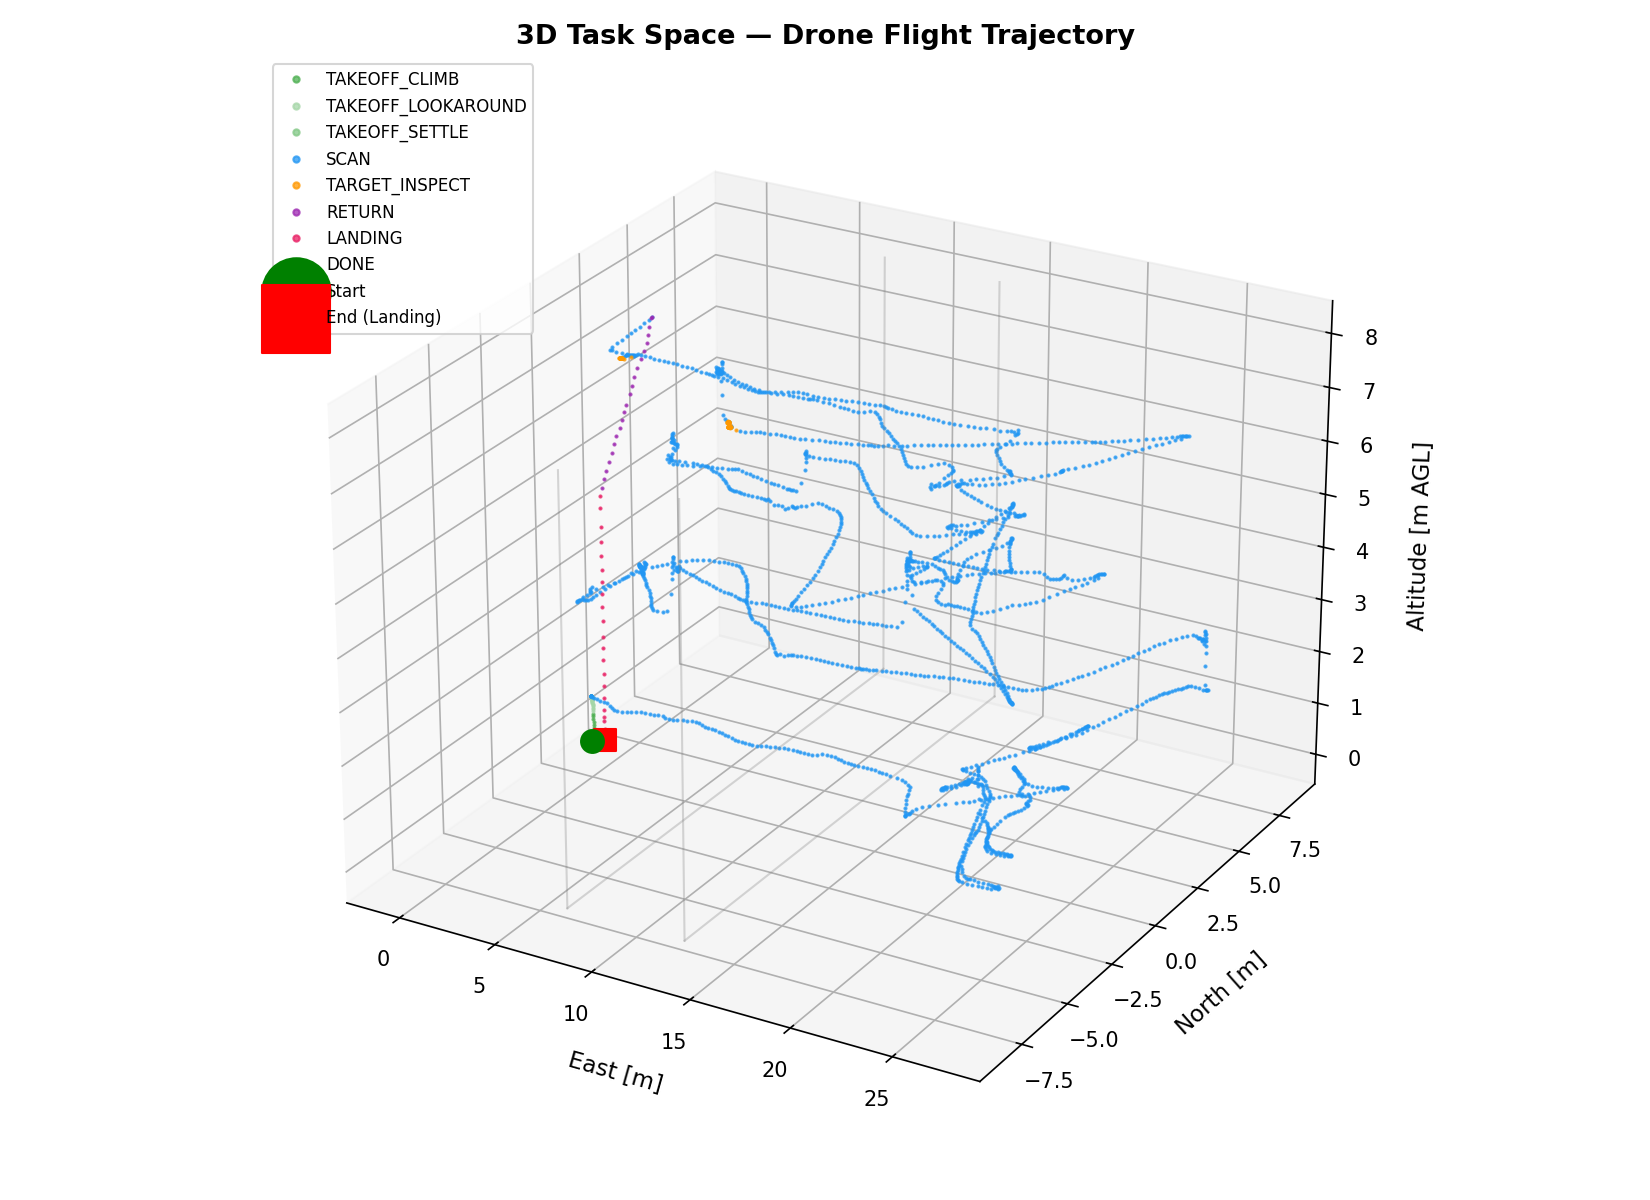
\includegraphics[width=0.75\textwidth]{../results/drone_3d_trajectory.png}
    \caption{מסלול הרחפן בתלת-ממד (N, E, Alt). כל מצב ב-\textenglish{FSM} מוצג בצבע שונה. נצפות בבירור 8 שכבות הגובה כ"מדרגות" אופקיות. הרחפן חצה מחדר A דרך המסדרון לחדר B.}
    \label{fig:drone_3d_trajectory}
\end{figure}

\begin{figure}[h]
    \centering
    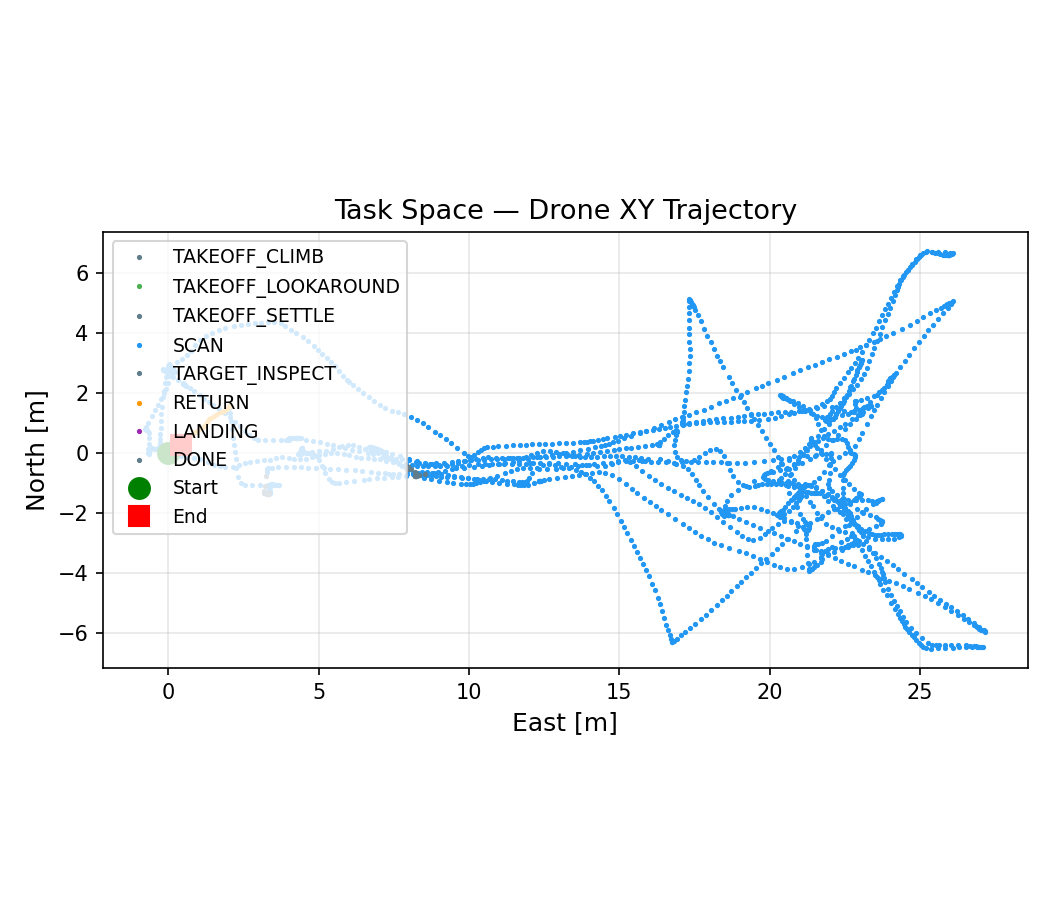
\includegraphics[width=0.55\textwidth]{../results/drone_task_xy.png}
    \caption{מסלול הרחפן במרחב המשימה — מבט עליון (XY ב-NED). הנקודה הירוקה — נקודת ההתחלה; האדומה — נקודת הסיום. הרחפן כיסה את חדר A, עבר דרך המסדרון ונכנס לחדר B.}
    \label{fig:drone_task_xy}
\end{figure}

\begin{figure}[h]
    \centering
    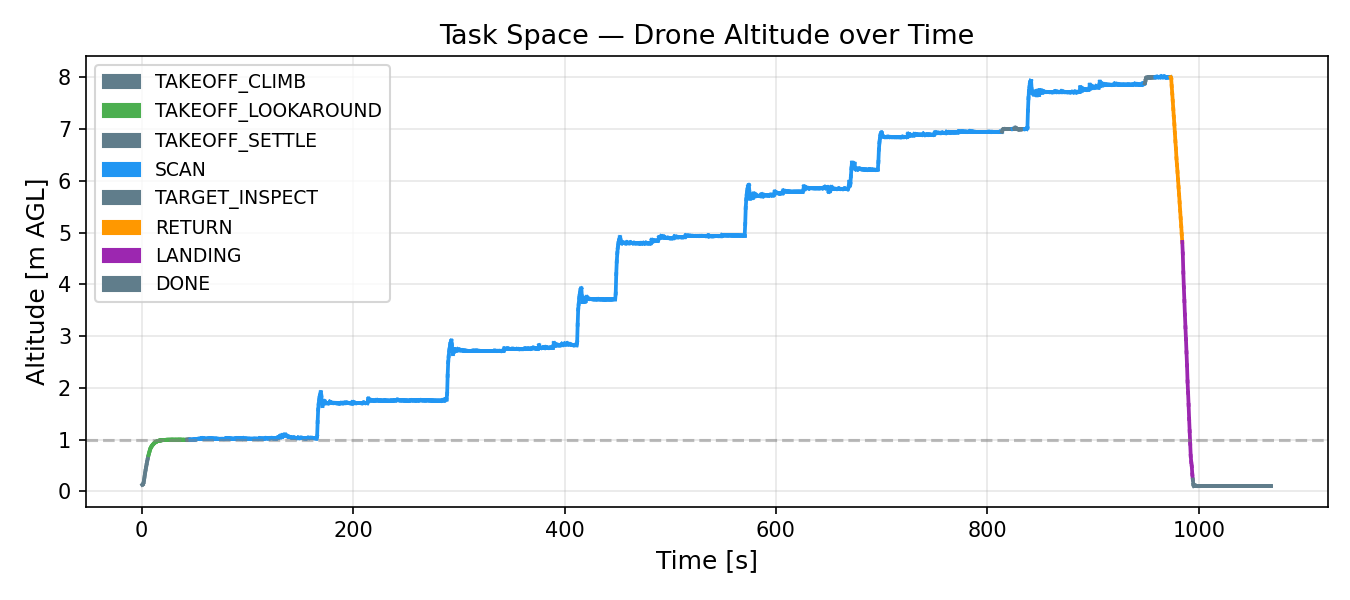
\includegraphics[width=0.80\textwidth]{../results/drone_task_altitude.png}
    \caption{גובה הרחפן כפונקציה של זמן. שמונה שכבות הסריקה מזוהות בבירור כ"מדרגות" חלקות. ירידה בסוף לנחיתה. ללא שלב \textenglish{TAKEOFF\_LOOKAROUND} — הרחפן עולה ישירות ל-\textenglish{SCAN}.}
    \label{fig:drone_task_altitude}
\end{figure}

\begin{figure}[h]
    \centering
    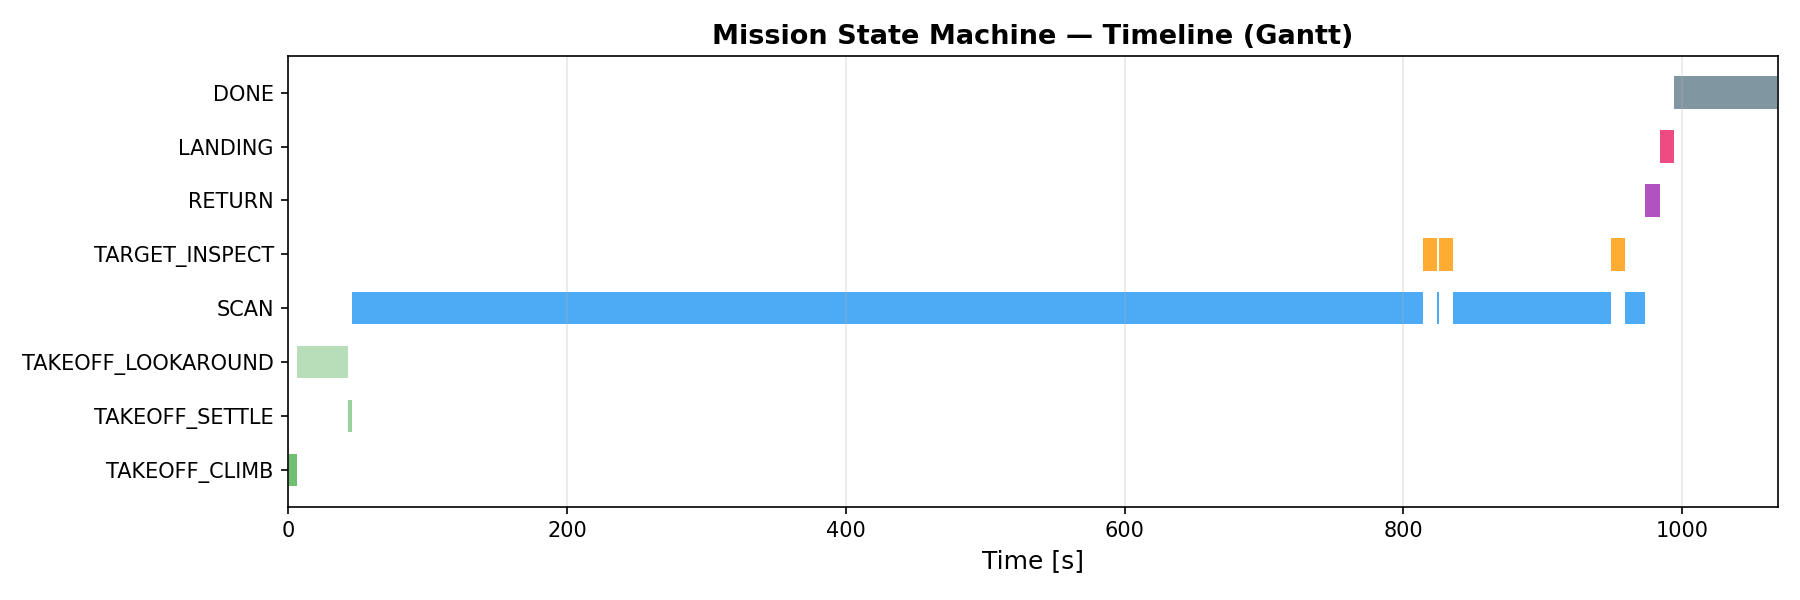
\includegraphics[width=0.80\textwidth]{../results/drone_state_gantt.png}
    \caption{ציר זמן מצבי מכונת המצבים (גאנט). שלושה מקטעי \textenglish{TARGET\_INSPECT} מזוהים (איתור 3 עצמים). \textenglish{SCAN} מהווה את מרבית זמן המשימה ($\approx$1000 שניות).}
    \label{fig:drone_state_gantt}
\end{figure}

\begin{figure}[h]
    \centering
    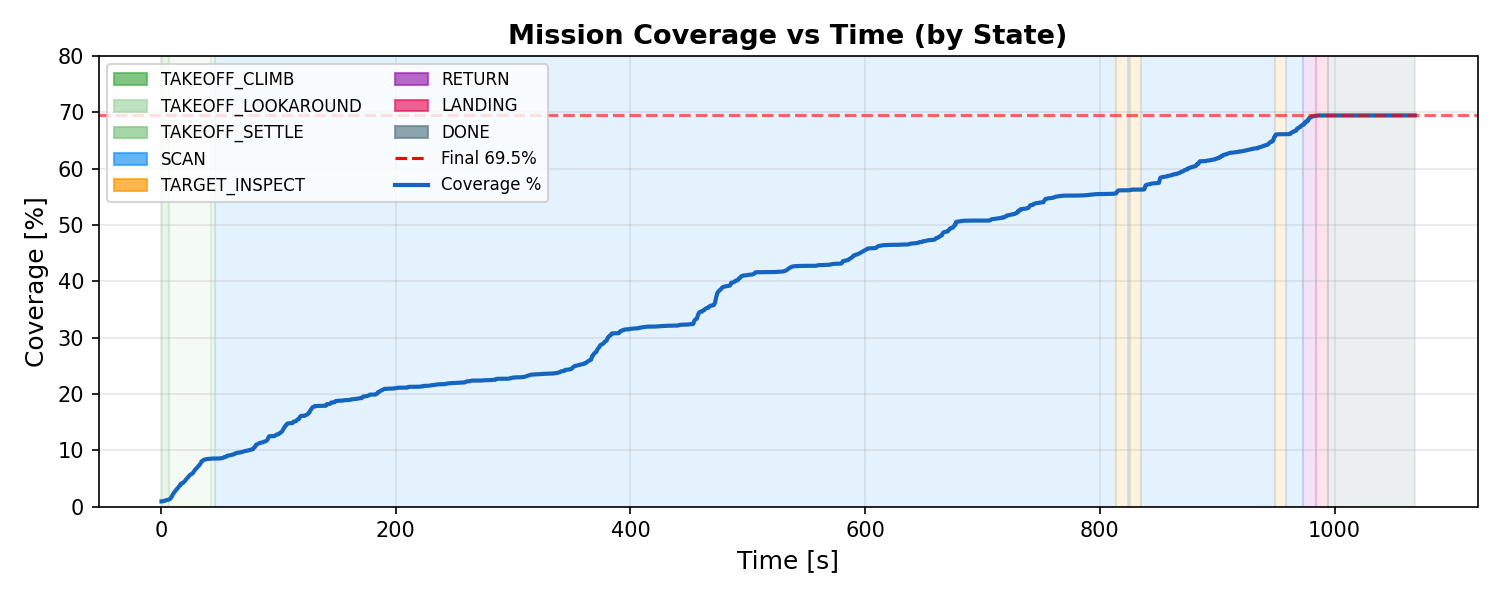
\includegraphics[width=0.80\textwidth]{../results/drone_coverage_timeline.png}
    \caption{כיסוי שטח (\%) לאורך הזמן עם צביעה לפי מצב. גידול יציב לאורך המשימה; עצירות קצרות במהלך \textenglish{TARGET\_INSPECT}. כיסוי סופי: \textbf{69.5\%}.}
    \label{fig:drone_coverage_timeline}
\end{figure}

\begin{figure}[h]
    \centering
    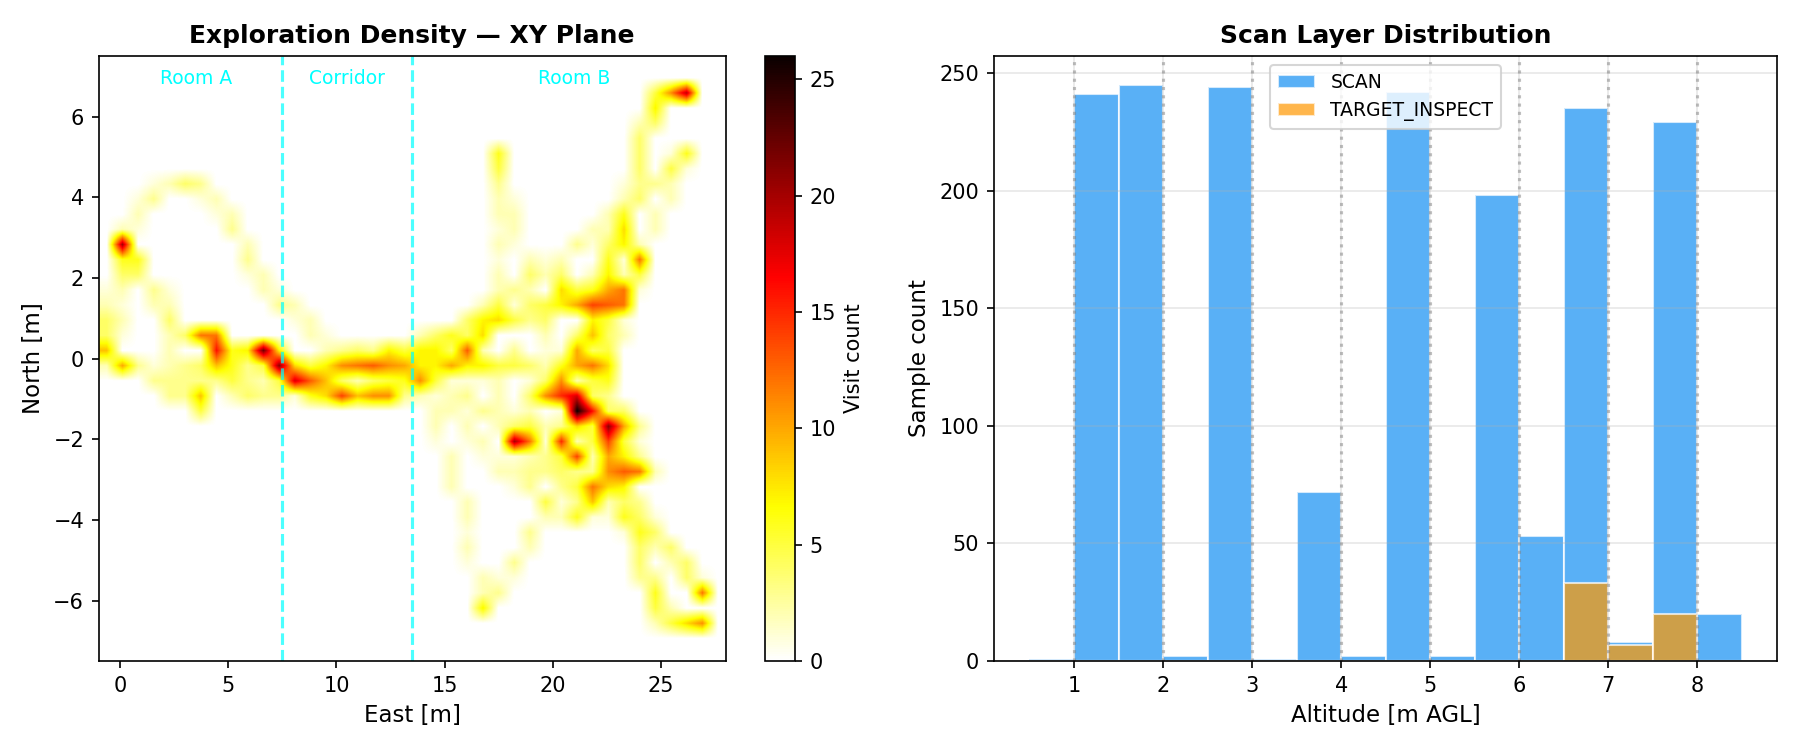
\includegraphics[width=0.85\textwidth]{../results/drone_exploration_density.png}
    \caption{\textbf{שמאל:} צפיפות חקר במישור XY — כיסוי גבוה בחדר A, חלקי במסדרון, כניסה לחדר B. \textbf{ימין:} התפלגות שכבות הגובה — כל 8 שכבות נוכחות בנתוני \textenglish{SCAN}.}
    \label{fig:drone_exploration_density}
\end{figure}

\subsection{תוצאות — מרחב הקונפיגורציה}

מרחב הקונפיגורציה של מערכת הרחפן מיוצג על-ידי מצב ה-\textenglish{VFH}: כיוון הניווט הנבחר ומספר הסקטורים החסומים.

\begin{figure}[h]
    \centering
    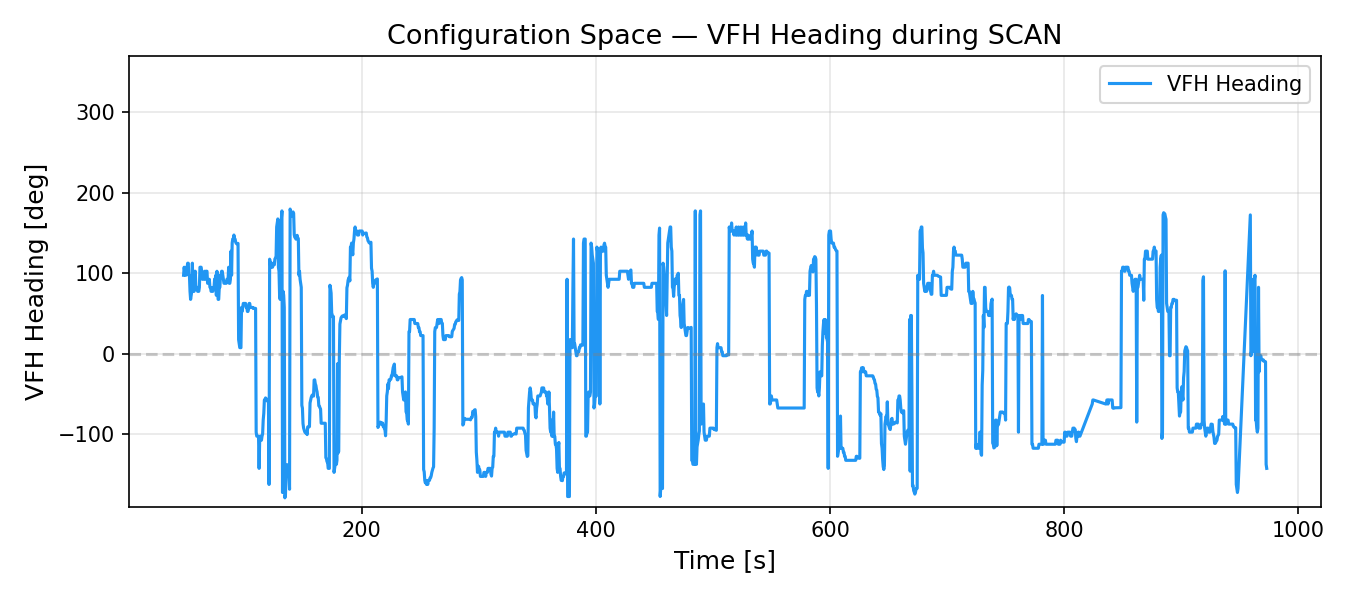
\includegraphics[width=0.80\textwidth]{../results/drone_config_heading.png}
    \caption{כיוון ה-\textenglish{VFH} הנבחר (במעלות) לאורך שלב ה-\textenglish{SCAN}. תנודות של $\pm 150^{\circ}$ מייצגות תגובה מהירה לסביבה המשתנה. במצב הולונומי, שינויי כיוון \textenglish{VFH} אינם גוררים סיבוב הרחפן — מה שמנע את סחיפת ה-\textenglish{SLAM}.}
    \label{fig:drone_config_heading}
\end{figure}

\begin{figure}[h]
    \centering
    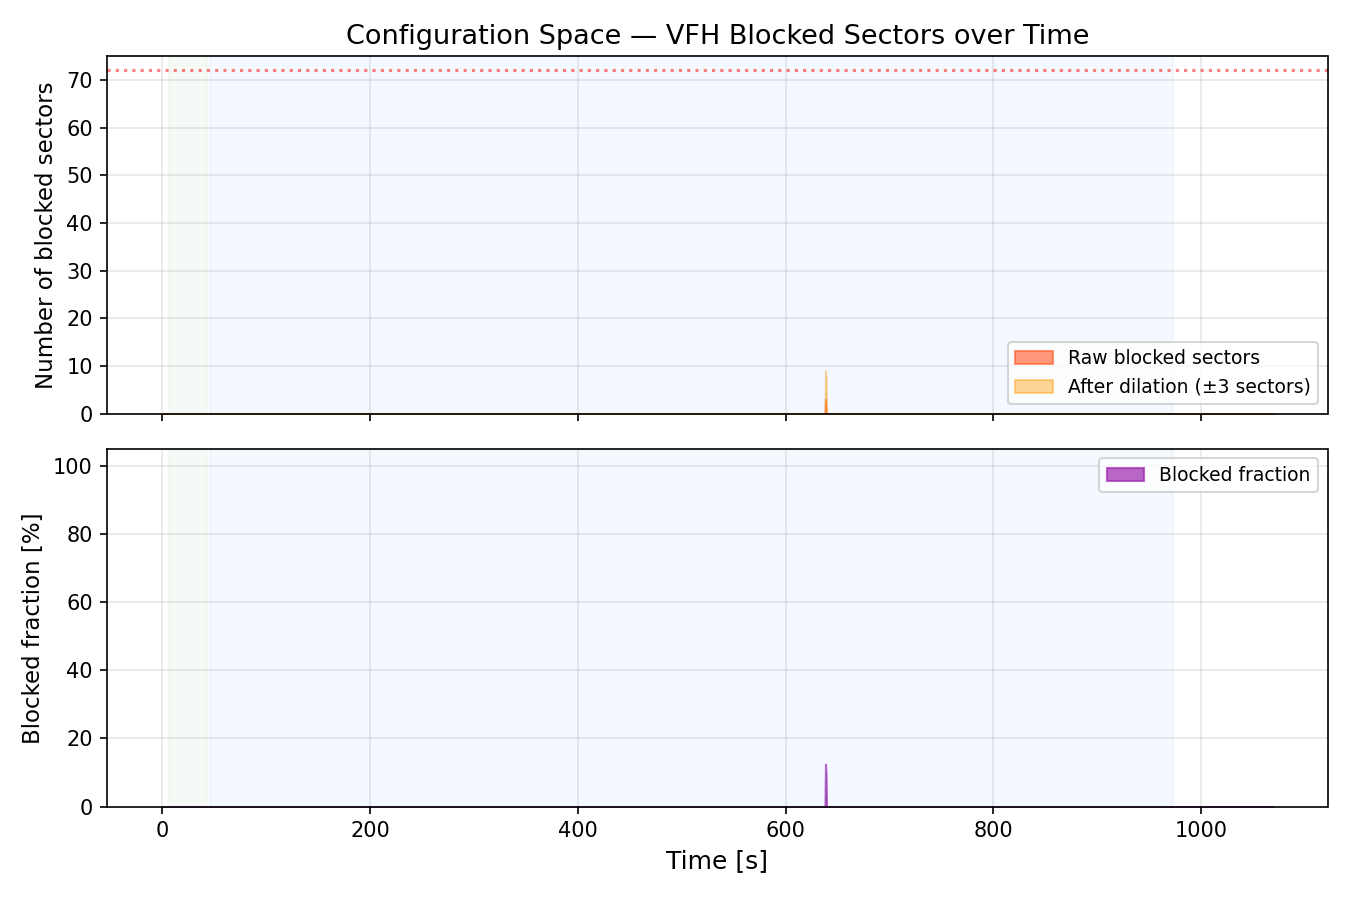
\includegraphics[width=0.80\textwidth]{../results/drone_config_sectors.png}
    \caption{למעלה: מספר סקטורי ה-\textenglish{VFH} החסומים (גולמי ולאחר הרחבה של $\pm 3$). למטה: אחוז הסקטורים החסומים. ערכים נמוכים לאורך מרבית המשימה — סביבה פתוחה; עליות ב-\textenglish{TARGET\_INSPECT} עם ההתקרבות לעצם.}
    \label{fig:drone_config_sectors}
\end{figure}

\section{משאבי הפרויקט — קבצים, וידאו והתקנה}

\subsection{מאגר הקוד (\textenglish{GitHub})}
\label{sec:links}

כל חומרי ההגשה — קוד המקור של שני החלקים, המצגת שהוצגה בכיתה (\texttt{\textenglish{FUEL.pptx}}), עותק המאמר, סרטוני הסימולציה, הגרפים וקובצי הנתונים — זמינים במאגר ה-\textenglish{GitHub}:

\begin{center}
\href{\repourl}{\repotext}
\end{center}

\begin{table}[H]
\centering
\begin{tabular}{cc}
\toprule
\textbf{נתיב במאגר} & \textbf{תוכן} \\
\midrule
\texttt{\textenglish{src/}} & חלק 1 — חבילות \textenglish{ROS2} של הזרוע (\textenglish{\texttt{my\_robot\_*}}) \\
\texttt{\textenglish{swarm\_project/ros2\_ws/src/}} & חלק 2 — חבילות \textenglish{ROS2} של הרחפן (\textenglish{\texttt{swarm\_*}}) \\
\texttt{\textenglish{results/}} & גרפים, קובצי נתונים (\textenglish{CSV}) וסרטוני הסימולציה \\
\texttt{\textenglish{review\_main/}} & מקור ה-\textenglish{LaTeX} של דו"ח זה \\
\texttt{\textenglish{FUEL.pptx}} & המצגת שהוצגה בכיתה \\
\texttt{\textenglish{Submission/}} & מסמך ההגשה המאוחד (דו"ח + נספחים) \\
\bottomrule
\end{tabular}
\caption{מבנה מאגר הקוד וחומרי ההגשה ב-\textenglish{GitHub}.}
\label{tab:repo_layout}
\end{table}

הוראות התקנה והרצה מפורטות, כולל תיעוד מלא של כל פונקציה, נמצאות בקובץ ה-\texttt{\textenglish{README.md}} שבתיקיית השורש של המאגר.

\subsection{עותק המאמר הנבחר}

המאמר עליו מבוסס חלק זה:

\begin{quote}
\textenglish{Zhou, B., Zhang, J., Chen, X., Xu, C., \& Gao, F. (2021). \textit{FUEL: Fast UAV Exploration Using Incremental Frontier Structure and Hierarchical Planning}. IEEE Robotics and Automation Letters, 6(2), 779–786. \texttt{DOI: 10.1109/LRA.2021.3051563}}
\end{quote}

עותק \textenglish{PDF} מלא של המאמר מצורף כנספח ב' בסוף מסמך זה, וזמין גם במאגר ה-\textenglish{GitHub}.

\subsection{קישורים לסרטוני הסימולציה}

שני סרטונים כלולים בתיקיית \texttt{\textenglish{results/}} שבמאגר:

\textbf{חלק 1 — הזרוע הרובוטית} (\href{\repourl/blob/main/results/arm_gazebo_demo.mp4}{\textenglish{\texttt{results/arm\_gazebo\_demo.mp4}}}, 1:12 דק'):
\begin{itemize}
    \item הרצת \texttt{\textenglish{playback.launch.py}} — השמעת מסלול ה-\textenglish{CTC+PID} ב-\textenglish{Gazebo}
    \item משימת \textenglish{Pick-and-Place} בין שני מדפים ללא התנגשות
    \item תצוגת המודל ב-\textenglish{RViz}
\end{itemize}

\textbf{חלק 2 — הרחפן האוטונומי} (\href{\repourl/blob/main/results/drone_swarm_mission_run.mp4}{\textenglish{\texttt{results/drone\_swarm\_mission\_run.mp4}}}, 18:25 דק'):
\begin{itemize}
    \item סביבת \textenglish{Gazebo}: חדר A + מסדרון + חדר B עם מכשולים
    \item לוח בקרת המשימה: מפת ה-\textenglish{voxel} התלת-ממדית המתעדכנת בזמן-אמת + \textenglish{frontier\_path}
    \item משימה מלאה: המראה $\rightarrow$ סריקה רב-שכבתית $\rightarrow$ איתור 3 מטרות $\rightarrow$ חזרה ונחיתה
\end{itemize}

\subsection{מבנה התוכנה והוראות התקנה}

\textbf{מבנה התוכנה — פונקציות עיקריות:}
\begin{table}[H]
\centering
\small
\begin{tabular}{ccc}
\toprule
\textbf{קובץ} & \textbf{שפה} & \textbf{פונקציות עיקריות} \\
\midrule
\texttt{\textenglish{voxel\_mapper.cpp}} & \textenglish{C++} & \textenglish{integrateDepth(), computeFrontiers(), planAstar()} \\
\texttt{\textenglish{search\_mission\_controller.cpp}} & \textenglish{C++} & \textenglish{compute\_vfh(), fsmUpdate(), publish\_velocity\_sp()} \\
\texttt{\textenglish{slam\_to\_px4.py}} & \textenglish{Python} & \textenglish{yaw-gate filtering (2 bad / 15 good)} \\
\texttt{\textenglish{dynamics.py}} & \textenglish{Python} & \textenglish{\_derive\_symbolic(), \_lambdify\_all()} \\
\texttt{\textenglish{controllers.py}} & \textenglish{Python} & \textenglish{ComputedTorquePID.step(), quintic\_trajectory()} \\
\texttt{\textenglish{navigation.py}} & \textenglish{Python} & \textenglish{biRRT(), check\_clearance()} \\
\bottomrule
\end{tabular}
\caption{הקבצים המרכזיים בקוד ופונקציותיהם העיקריות.}
\label{tab:main_functions}
\end{table}

\textbf{דרישות מקדימות:}
\begin{itemize}
    \item \textenglish{Ubuntu 24.04 LTS}
    \item \textenglish{ROS 2 Jazzy Jalisco} (Full desktop install)
    \item \textenglish{Gazebo Harmonic}
    \item \textenglish{PX4 Autopilot v1.14} (SITL) — לחלק 2 בלבד
    \item \textenglish{Python 3.11} + חבילות: \texttt{\textenglish{numpy, scipy, sympy, matplotlib, pandas}}
\end{itemize}

\textbf{הוראות התקנה והרצה — חלק 1 (זרוע):}
\begin{enumerate}
    \item \texttt{\textenglish{pip install numpy scipy sympy matplotlib}}
    \item \texttt{\textenglish{colcon build --symlink-install}} ואז \texttt{\textenglish{source install/setup.bash}} (מתיקיית השורש של המאגר)
    \item \texttt{\textenglish{python3 -m my\_robot\_control.simulate\_free}} \; — תגובה חופשית + גרפים
    \item \texttt{\textenglish{python3 -m my\_robot\_control.simulate\_pid}} \; — בקר \textenglish{CTC+PID} + גרפים
    \item \texttt{\textenglish{ros2 launch my\_robot\_control playback.launch.py}} \; — הדגמה מלאה ב-\textenglish{Gazebo}
\end{enumerate}

\textbf{הוראות התקנה והרצה — חלק 2 (רחפן):}
\begin{enumerate}
    \item הגדר \textenglish{PX4 SITL} לפי \texttt{\textenglish{docs.px4.io/main/en/simulation/}} והפעל \texttt{\textenglish{MicroXRCEAgent udp4 -p 8888}}
    \item \texttt{\textenglish{cd swarm\_project/ros2\_ws \&\& colcon build --symlink-install}}
    \item \texttt{\textenglish{source install/setup.bash}}
    \item \texttt{\textenglish{make px4\_sitl gz\_x500}} (מתיקיית \textenglish{PX4-Autopilot})
    \item \texttt{\textenglish{ros2 launch swarm\_bringup d1\_single\_agent\_search.launch.py}}
\end{enumerate}

זמן הרצה משוער למשימת חקר מלאה: \textasciitilde{}15-20 דקות (תלוי בגיאומטריית הסביבה).

\section{מסקנות}

\subsection{מה בוצע — סיכום שינויים עיקריים}

\begin{table}[H]
\centering
\small
\begin{tabular}{ccc}
\toprule
\textbf{בעיה} & \textbf{סיבת שורש} & \textbf{פתרון} \\
\midrule
קריסת \textenglish{Gazebo} & חסר \textenglish{executable bit} לסקריפט & \texttt{chmod +x} \\
מריחת \textenglish{SLAM} & סיבוב 360$^{\circ}$ בהמראה & \texttt{takeoff\_lookaround\_enabled: False} \\
מריחת \textenglish{SLAM} & שני חיישנים כותבים למפה & \texttt{integrate\_lidar\_into\_map: False} \\
מריחת \textenglish{SLAM} & \textenglish{log-odds} גבוה מדי (רעש) & שינוי $l_{hit}$ מ-0.85 ל-0.60 \\
\textenglish{Yaw} oscillation & \textenglish{VFH} מחייב סיבוב לפני תנועה & \textenglish{VFH} הולונומי: \textenglish{yaw} מנותק \\
\textenglish{RTAB-Map} drift & \textenglish{motion blur} בסיבוב מהיר & נזנח; \textenglish{PX4 EKF2} בלבד \\
\bottomrule
\end{tabular}
\caption{סיכום הבעיות שאובחנו במהלך הפיתוח, סיבות השורש והפתרונות שיושמו.}
\label{tab:problems_solutions}
\end{table}

\subsection{יתרונות הגישה}

\begin{itemize}
    \item \textbf{עדכון מצטבר — השראת \textenglish{FUEL}}: כמו ה-\textenglish{FIS} של \textenglish{FUEL}, מתעדכנים רק האשכולות שהמפה השתנתה בסביבתם — עלות $O(\Delta N)$ במקום $O(N)$ כולל. זה מאפשר ריצה בזמן-אמת ב-2 \textenglish{Hz} גם עבור מרחבים גדולים.

    \item \textbf{תכנון \textenglish{A*} מהיר ובטוח}: \textenglish{A*} עם עונש \textenglish{Voronoi} מוצא נתיבים המרוחקים ממכשולים ומותאמים לסביבה פיזית — בעלות חישובית $O(V \log V)$, הרבה יותר נמוכה מ-\textenglish{ATSP}.

    \item \textbf{\textenglish{VFH} הולונומי}: ניתוק ה-\textenglish{yaw} מכיוון התנועה מבטל את בעיית ה-\textenglish{SLAM drift} שנגרמה מסיבובים מהירים. הרחפן נע בכיוון ה-\textenglish{VFH} ישירות ב-72 כיוונים אפשריים.

    \item \textbf{חיישן יחיד}: הסרת ה-\textenglish{LiDAR} פישטה את הארכיטקטורה — פחות משקל, פחות חיבורים, אין קונפליקטים בין חיישנים. \textenglish{OAK-D Lite} מספק מיפוי ו-\textenglish{VFH} מאותו מקור.

    \item \textbf{סינון השער ב-\textenglish{slam\_to\_px4}}: שכבת ההיסטרזיס (2 bad / 15 good) מגנה מסחיפת \textenglish{yaw} תוך שמירה על רציפות הניווט. כשהשער פעיל — \textenglish{EKF2} ממשיך ב-\textenglish{IMU} בלבד למשך פחות מ-750 מילישניות.

    \item \textbf{ניקוד מושכל}: משקלי מידע, מרווח, מרחק והתקדמות בניקוד נקודות התצפית מכוונים את הרחפן לאזורים בעלי ערך חקר גבוה — בדומה לעקרון ה-\textenglish{viewpoint refinement} של \textenglish{FUEL}.
\end{itemize}

\subsection{התאמות הנדסיות — בחירות מכוונות וטרייד-אופים}

הגישה שנבחרה כוללת מספר הסתגלויות מכוונות ביחס ל-\textenglish{FUEL} המקורי, כל אחת עם רציונל הנדסי ברור:

\begin{itemize}
    \item \textbf{בחירה: \textenglish{A*} במקום \textenglish{ATSP}}: אלגוריתם \textenglish{A*} עם עונש \textenglish{Voronoi} (ריכוז הנתיב במרכז המסדרון) הוכח ככלי תכנון גלובלי מספק לסביבות של חדרים ומסדרונות. \textenglish{ATSP} יניב יעילות מסלול גבוהה יותר בסביבות רב-חדריות עם עשרות אשכולות — אולם מצריך ספריית \textenglish{TSP} חיצונית (\textenglish{LKH / OR-Tools}) ותקציב חישובי גדול יותר. הרחבה זו מתוכננת לשלב הבא.

    \item \textbf{בחירה: \textenglish{VFH} הולונומי במקום \textenglish{B-spline}}: הרחפן \textenglish{X500} עם \textenglish{PX4 Offboard} יכול לבצע תנועה הולונומית מלאה — ה-\textenglish{VFH} ההולונומי מנצל זאת ישירות. \textenglish{VFH} מספק הימנעות ממכשולים בזמן-אמת (72 סקטורים $\times$ 10 \textenglish{Hz}) עם עלות חישובית זניחה. \textenglish{B-spline} מינימום-זמן יאפשר מהירויות גבוהות יותר (2-3 מ'/ש' לעומת $v_{max}=0.7$ מ'/ש' כיום), אך דורש שילוב \textenglish{MPC} לאכיפת מגבלות דינמיות — עבודה עתידית.

    \item \textbf{מגבלה טכנית — מסדרונות צרים}: ניפוח מכשולים של תא אחד (0.2 מ') עלול "לנתק" את ה-\textenglish{BFS} מאשכולות גבול הסמוכים לעמודים צרים. הפחתת \texttt{obstacle\_inflate\_cells} מ-2 ל-1 שיפרה זאת משמעותית. מגבלה זו ניתנת לתיקון מלא באמצעות \textenglish{Bresenham corridor dilation} לאורך ציר המסדרון.

    \item \textbf{הרחבה לנחיל}: הארכיטקטורה מתוכננת ל-\textenglish{swarm}: חבילת \texttt{\textenglish{swarm\_coordination}} קיימת כבר ב-\textenglish{workspace}; שיתוף מפות \textenglish{log-odds} בין רחפנים וחלוקת אשכולות \textenglish{FIS} מהווים את שלב הפיתוח הבא.
\end{itemize}

\subsection{המלצות לעתיד}

\begin{itemize}
    \item \textbf{יישום \textenglish{ATSP} מלא}: הוספת מודול פתרון \textenglish{TSP} (למשל \textenglish{LKH} או \textenglish{OR-Tools}) על כל אשכולות ה-\textenglish{FIS} — לחיסכון מוערך של 30-50\% במסלול.

    \item \textbf{מסלול \textenglish{B-spline}}: החלפת ניווט \textenglish{A*}+\textenglish{VFH} ב-\textenglish{B-spline} מינימום-זמן + \textenglish{MPC} לאחר גילוי יעד.

    \item \textbf{גבולות תלת-ממדיים}: השימוש במפת הווקסל התלת-ממדית (הקיימת כבר ב-\textenglish{voxel\_mapper}) לגילוי גבולות 3D — כמו \textenglish{FUEL} המקורי.

    \item \textbf{הרחבה לנחיל}: שיתוף מפות \textenglish{log-odds} בין מספר רחפנים וחלוקת אשכולות ה-\textenglish{FIS} ביניהם — למקסום כיסוי מקבילי ולמניעת כפילויות.
\end{itemize}

% ==================== סוף חלק 2 ====================

% ==================== נספחים ====================
\clearpage
\phantomsection
\addcontentsline{toc}{part}{נספחים}
\part*{נספחים}

\noindent מסמך זה כולל שני נספחים:
\begin{itemize}
    \item \textbf{נספח א'} — המצגת שהוצגה בכיתה ב-1.7.2026 (13 שקפים; הקובץ המקורי: \texttt{\textenglish{FUEL.pptx}} במאגר).
    \item \textbf{נספח ב'} — עותק מלא של המאמר הנבחר: \textenglish{Zhou et al., \textit{FUEL: Fast UAV Exploration Using Incremental Frontier Structure and Hierarchical Planning}, IEEE RA-L 2021}.
\end{itemize}

% — נספח א' — המצגת שהוצגה בכיתה —
\clearpage
\phantomsection
\addcontentsline{toc}{section}{נספח א' — המצגת שהוצגה בכיתה}
\includepdf[pages=-,landscape=true]{fuel_slides.pdf}

% — נספח ב' — עותק המאמר —
\clearpage
\phantomsection
\addcontentsline{toc}{section}{נספח ב' — עותק המאמר (FUEL, IEEE RA-L 2021)}
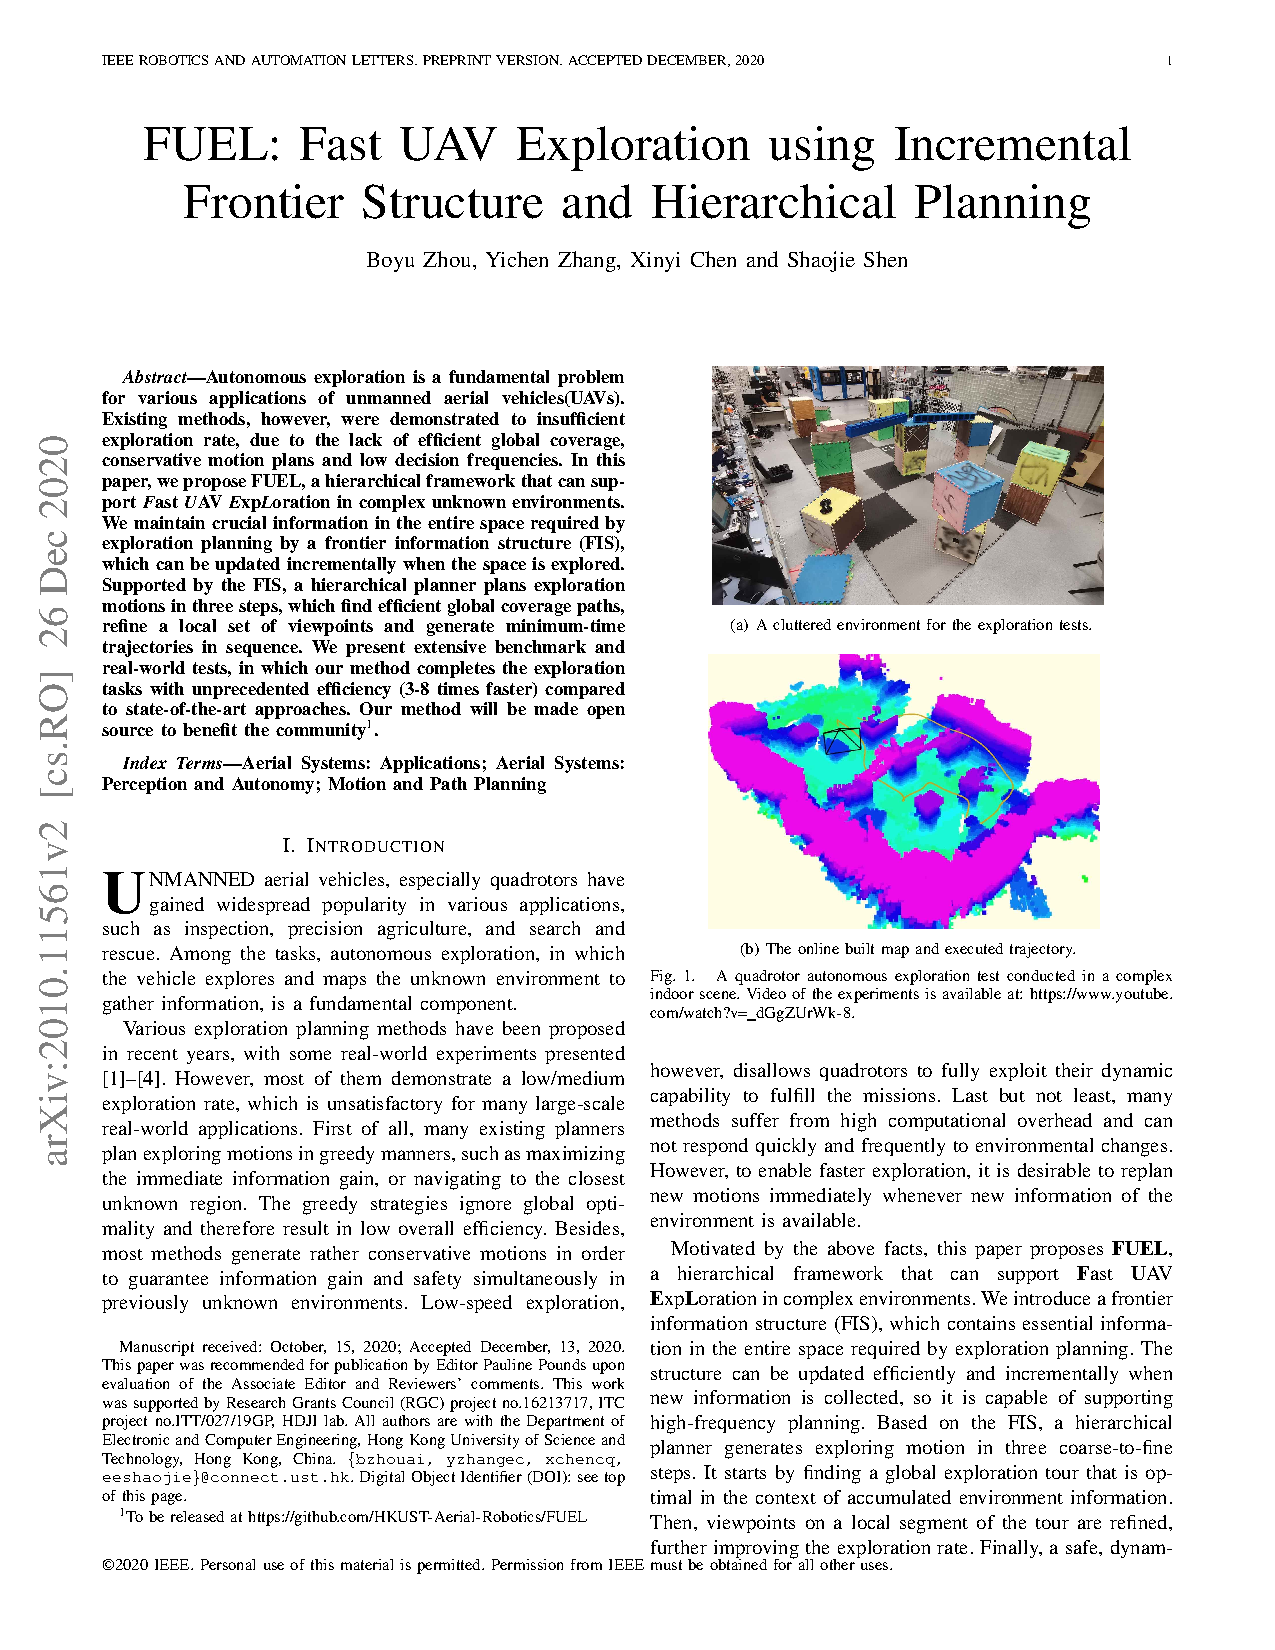
\includepdf[pages=-]{fuel_paper.pdf}

\end{document}